\documentclass[oneside,openany,phd]{TMU-Thesis}


% ==================== structure/preamble.tex ====================
% مشخصات پایان‌نامه را در فایلهای faTitle و enTitle وارد نمایید.
% در اینجا برای یکپارچگی، همینجا وارد می‌کنیم

% مشخصات فارسی
\university{تربیت مدرس}
\faculty{مهندسی برق و کامپیوتر}
\department{گروه هوش مصنوعی و رباتیکز}
\subject{مهندسی کامپیوتر}
\field{مهندسی نرم‌افزار}
\credits{---} % در رساله دکتری معمولا به صورت واحدی ذکر نمی‌شود یا فیلد خالی است
\title{یادگیری تقویتی عمیق با شکل‌دهی تصادفی پاداش برای مدیریت عدم قطعیت در سیستم‌های خودوفقی}
\firstsupervisor{دکتر ...}
% \secondsupervisor{استاد راهنمای دوم}
\firstadvisor{دکتر ...}
% \secondadvisor{استاد مشاور دوم}
\name{علیرضا}
\surname{کاویانی‌فر}
\studentID{...}
\thesisdate{بهمن ۱۴۰۴}

% مشخصات انگلیسی
\latinuniversity{Tarbiat Modares University}
\latinfaculty{Faculty of Electrical and Computer Engineering}
\latinsubject{Computer Engineering}
\latinfield{Software Engineering}
\latintitle{Randomized Reward-Shaped Deep Reinforcement Learning for Managing Uncertainty in Self-Adaptive Systems}
\firstlatinsupervisor{Dr. ...}
\firstlatinadvisor{Dr. ...}
\latinname{Alireza}
\latinsurname{Kavianifar}
\latinthesisdate{February 2026}
\latinkeywords{Self-Adaptive Systems, Deep Reinforcement Learning, Randomized Reward Shaping, Uncertainty Management, Formal Verification, UPPAAL-SMC}

% فراخوانی بسته‌ها و دستورات استاندارد
% در این فایل، دستورها و تنظیمات مورد نیاز، آورده شده است.
%-------------------------------------------------------------------------------------------------------------------

% در ورژن جدید زی‌پرشین برای تایپ متن‌های ریاضی، این سه بسته، حتماً باید فراخوانی شود
\usepackage{amsthm,amssymb,amsmath}
% بسته‌ای برای تنطیم حاشیه‌های بالا، پایین، چپ و راست صفحه
\usepackage[top=30mm, bottom=25mm, left=25mm, right=35mm]{geometry}
% بسته‌‌ای برای ظاهر شدن شکل‌ها و تصاویر متن
\usepackage{graphicx}
% بسته‌ای برای رسم کادر
\usepackage{framed} 
% بسته‌‌ای برای چاپ شدن خودکار تعداد صفحات در صفحه «معرفی پایان‌نامه»
\usepackage{lastpage}
% بسته‌ و دستوراتی برای ایجاد لینک‌های رنگی با امکان جهش
% \usepackage[pagebackref=false,colorlinks,linkcolor=black,citecolor=black]{hyperref}
% چنانچه قصد پرینت گرفتن نوشته خود را دارید، خط بالا را غیرفعال و  از دستور زیر استفاده کنید چون در صورت استفاده از دستور زیر‌‌، 
% لینک‌ها به رنگ سیاه ظاهر خواهند شد که برای پرینت گرفتن، مناسب‌تر است
% \usepackage[pagebackref=false]{hyperref}
% بسته‌ لازم برای تنظیم سربرگ‌ها
\usepackage{fancyhdr}
\setlength{\headheight}{16pt}
%
\usepackage{setspace}
\usepackage{algorithm}
\usepackage{algorithmic}
\usepackage{subfigure}
\usepackage[subfigure]{tocloft}
\usepackage{multirow}


% بسته‌ای برای ظاهر شدن «مراجع» و «نمایه» در فهرست مطالب
\usepackage[nottoc]{tocbibind}
% دستورات مربوط به ایجاد نمایه
\usepackage{makeidx}
\makeindex
% تعریف شیم‌های مورد نیاز برای نسخه‌های جدید بسته bidi در برخی محیط‌ها
% Removal of redundant and potentially broken definitions
\makeatletter
% شیم‌های سازگاری برای نسخه‌های جدید لاتک و بسته‌های bidi/xepersian
\providecommand{\IfClassLoadedT}[2]{\@ifclassloaded{#1}{#2}{}}
\providecommand{\IfClassLoadedF}[2]{\@ifclassloaded{#1}{}{#2}}
\providecommand{\IfClassLoadedTF}[3]{\@ifclassloaded{#1}{#2}{#3}}
\providecommand{\IfPackageLoadedT}[2]{\@ifpackageloaded{#1}{#2}{}}
\providecommand{\IfPackageLoadedF}[2]{\@ifpackageloaded{#1}{}{#2}}
\providecommand{\IfPackageLoadedTF}[3]{\@ifpackageloaded{#1}{#2}{#3}}
\providecommand{\@iffileloaded}[3]{\expandafter\ifx\csname ver@#1\endcsname\relax#3\else#2\fi}
\providecommand{\IfFileLoadedT}[2]{\@iffileloaded{#1}{#2}{}}
\providecommand{\IfFileLoadedF}[2]{\@iffileloaded{#1}{}{#2}}
\providecommand{\IfFileLoadedTF}[3]{\@iffileloaded{#1}{#2}{#3}}
\makeatother

%%%%%%%%%%%%%%%%%%%%%%%%%%
% فراخوانی بسته زی‌پرشین و تعریف قلم فارسی و انگلیسی
\usepackage[pagebackref=false,colorlinks,linkcolor=black,citecolor=black]{hyperref}
\usepackage{notoccite}

\ExplSyntaxOn
\cs_if_exist:NTF \g__hyp_linknestlevel_int { } { \int_new:N \g__hyp_linknestlevel_int }
\cs_if_exist:NTF \l__hyp_annot_GoTo_bool { } { \bool_new:N \l__hyp_annot_GoTo_bool }
\cs_if_exist:NTF \l__hyp_annot_URI_bool { } { \bool_new:N \l__hyp_annot_URI_bool }
\cs_if_exist:NTF \l__hyp_href_url_ismap_bool { } { \bool_new:N \l__hyp_href_url_ismap_bool }
\cs_if_exist:NTF \l__hyp_text_enc_uri_print_tl { } { \tl_new:N \l__hyp_text_enc_uri_print_tl }
\cs_if_exist:NTF \l__hyp_uri_tmpa_tl { } { \tl_new:N \l__hyp_uri_tmpa_tl }

% Defining missing l3pdf/pdfdict commands if not present
\cs_if_exist:NTF \pdfdict_put:nno { } { \cs_new:Npn \pdfdict_put:nno #1#2#3 { } }
\cs_if_exist:NTF \pdfdict_put:nnn { } { \cs_new:Npn \pdfdict_put:nnn #1#2#3 { } }
\cs_if_exist:NTF \pdfdict_use:n { } { \cs_new:Npn \pdfdict_use:n #1 { } }
\cs_if_exist:NTF \pdfannot_dict_put:nne { } { \cs_new:Npn \pdfannot_dict_put:nne #1#2#3 { } }
\cs_if_exist:NTF \pdfannot_link:nen { } { \cs_new:Npn \pdfannot_link:nen #1#2#3 { } }
\cs_if_exist:NTF \__hyp_check_link_nesting:TF { } { \cs_new:Npn \__hyp_check_link_nesting:TF #1#2 { #1 } }
\cs_if_exist:NTF \__hyp_text_pdfstring:eoN { } { \cs_new:Npn \__hyp_text_pdfstring:eoN #1#2#3 { } }
\ExplSyntaxOff

% تعریف دستورات گمشده برای جلوگیری از خطای renewcommand در بسته‌های داخلی
\makeatletter
\providecommand{\foottextfont}{}
\providecommand{\LTRfoottextfont}{}
\providecommand{\RTLfoottextfont}{}
\providecommand{\abstractname}{}
\providecommand{\latinabstract}{}
\providecommand{\AutoPersianDigits}{}
\makeatother

\usepackage{xepersian}
\settextfont[Path=font/,Extension=.ttf,Scale=1,
    BoldFont=XB NiloofarBd,
    ItalicFont=XB NiloofarIt,
    BoldItalicFont=XB NiloofarBdIt
]{XB Niloofar}
\setlatintextfont[Scale=0.9]{Times New Roman}

%%%%%%%%%%%%%%%%%%%%%%%%%%
% چنانچه می‌خواهید اعداد در فرمول‌ها، انگلیسی باشد، خط زیر را غیرفعال کنید
\setdigitfont[Path=font/,Extension=.ttf,Scale=1,
    BoldFont=XB NiloofarBd,
    ItalicFont=XB NiloofarIt,
    BoldItalicFont=XB NiloofarBdIt
]{XB Niloofar}
%%%%%%%%%%%%%%%%%%%%%%%%%%
% تعریف قلم‌های فارسی و انگلیسی اضافی برای استفاده در بعضی از قسمت‌های متن
\defpersianfont\titlefont[Path=font/,Extension=.ttf,Scale=1]{XB Titre}
% \defpersianfont\iranic[Scale=1.1]{XB Zar Oblique}%Italic}%
% \defpersianfont\nastaliq[Scale=1.2]{IranNastaliq}

%%%%%%%%%%%%%%%%%%%%%%%%%%
% دستوری برای حذف کلمه «چکیده»
\renewcommand{\abstractname}{}
% دستوری برای حذف کلمه «abstract»
%\renewcommand{\latinabstract}{}
% دستوری برای تغییر نام کلمه «اثبات» به «برهان»
\renewcommand\proofname{\textbf{برهان}}
% دستوری برای تغییر نام کلمه «کتاب‌نامه» به «مراجع»
\renewcommand{\bibname}{مراجع}
% دستوری برای تعریف واژه‌نامه انگلیسی به فارسی
\newcommand\persiangloss[2]{#1\dotfill\lr{#2}\\}
% دستوری برای تعریف واژه‌نامه فارسی به انگلیسی 
\newcommand\englishgloss[2]{#2\dotfill\lr{#1}\\}
% تعریف دستور جدید «\پ» برای خلاصه‌نویسی جهت نوشتن عبارت «پروژه/پایان‌نامه/رساله»
\newcommand{\پ}{پروژه/پایان‌نامه/رساله }

%\newcommand\BackSlash{\char`\\}

%%%%%%%%%%%%%%%%%%%%%%%%%%
\SepMark{-}

% تعریف و نحوه ظاهر شدن عنوان قضیه‌ها، تعریف‌ها، مثال‌ها و ...
\theoremstyle{definition}
\newtheorem{definition}{تعریف}[section]
\theoremstyle{plain}
\newtheorem{theorem}[definition]{قضیه}
\newtheorem{lemma}[definition]{لم}
\newtheorem{proposition}[definition]{گزاره}
\newtheorem{corollary}[definition]{نتیجه}
\newtheorem{remark}[definition]{ملاحظه}
\theoremstyle{definition}
\newtheorem{example}[definition]{مثال}

%\renewcommand{\theequation}{\thechapter-\arabic{equation}}
%\def\bibname{مراجع}
\numberwithin{algorithm}{chapter}
\def\listalgorithmname{فهرست الگوریتم‌ها}
\def\listfigurename{فهرست تصاویر}
\def\listtablename{فهرست جداول}

%%%%%%%%%%%%%%%%%%%%%%%%%%%%
% دستورهایی برای سفارشی کردن سربرگ صفحات
% \newcommand{\SetHeader}{
% \csname@twosidetrue\endcsname
% \pagestyle{fancy}
% \fancyhf{} 
% \fancyhead[OL,EL]{\thepage}
% \fancyhead[OR]{\small\rightmark}
% \fancyhead[ER]{\small\leftmark}
% \renewcommand{\chaptermark}[1]{%
% \markboth{\thechapter-\ #1}{}}
% }
%%%%%%%%%%%%5
%\def\MATtextbaseline{1.5}
%\renewcommand{\baselinestretch}{\MATtextbaseline}
\doublespacing
%%%%%%%%%%%%%%%%%%%%%%%%%%%%%
% دستوراتی برای اضافه کردن کلمه «فصل» و شماره ترتیبی حروفی در فهرست مطالب

\makeatletter
% سفارشی‌سازی عدد ۱ در سیستم ابجد برای نمایش کلمه «الف» به جای «آ»
\def\@abjad#1{%
\ifnum#1=1 الف%
\else
  \ifnum#1>1999 \xpg@warning{Illegal value (#1) for abjad numeral} {#1}%
  \else
    \ifnum#1<\z@\space\xpg@warning{Illegal value (#1) for abjad numeral}%
    \else
      \ifnum#1<10\expandafter\abj@num@i\number#1%
      \else
        \ifnum#1<100\expandafter\abj@num@ii\number#1%
        \else
          \ifnum#1<\@m\expandafter\abj@num@iii\number#1%
          \else
            \ifnum#1<\@M\expandafter\abj@num@iv\number#1%
            \fi
          \fi
        \fi
      \fi
    \fi
  \fi
\fi}
\def\abj@num@i#1{%
  \ifcase#1\or ا\or ب\or ج\or د%
           \or ه\or و\or ز\or ح\or ط\fi
  \ifnum#1=\z@\abjad@zero\fi}

\newcommand{\persianchapnum}[1]{%
  \edef\@arg{#1}%
  \def\@one{1}\def\@pone{۱}%
  \def\@two{2}\def\@ptwo{۲}%
  \def\@three{3}\def\@pthree{۳}%
  \def\@four{4}\def\@pfour{۴}%
  \def\@five{5}\def\@pfive{۵}%
  \def\@six{6}\def\@psix{۶}%
  \def\@seven{7}\def\@pseven{۷}%
  \def\@eight{8}\def\@peight{۸}%
  \def\@nine{9}\def\@pnine{۹}%
  \def\@ten{10}\def\@pten{۱۰}%
  \ifx\@arg\@one اول%
  \else\ifx\@arg\@pone اول%
  \else\ifx\@arg\@two دوم%
  \else\ifx\@arg\@ptwo دوم%
  \else\ifx\@arg\@three سوم%
  \else\ifx\@arg\@pthree سوم%
  \else\ifx\@arg\@four چهارم%
  \else\ifx\@arg\@pfour چهارم%
  \else\ifx\@arg\@five پنجم%
  \else\ifx\@arg\@pfive پنجم%
  \else\ifx\@arg\@six ششم%
  \else\ifx\@arg\@psix ششم%
  \else\ifx\@arg\@seven هفتم%
  \else\ifx\@arg\@pseven هفتم%
  \else\ifx\@arg\@eight هشتم%
  \else\ifx\@arg\@peight هشتم%
  \else\ifx\@arg\@nine نهم%
  \else\ifx\@arg\@pnine نهم%
  \else\ifx\@arg\@ten دهم%
  \else\ifx\@arg\@pten دهم%
  \else #1\fi\fi\fi\fi\fi\fi\fi\fi\fi\fi\fi\fi\fi\fi\fi\fi\fi\fi\fi\fi
}

\newlength\mylenprt
\newlength\mylenchp
\newlength\mylenapp

\renewcommand\cftpartpresnum{\partname~}
\renewcommand\cftchappresnum{\chaptername~}
\renewcommand\cftchapaftersnum{:}

\settowidth\mylenprt{\cftpartfont\cftpartpresnum\cftpartaftersnum}
% تنظیم پهنای کادر شماره متناسب با عریض‌ترین عنوان فصل («فصل چهارم: »)
\settowidth\mylenchp{\cftchapfont\chaptername~چهارم:\space}
\settowidth\mylenapp{\cftchapfont\appendixname~\cftchapaftersnum}
\addtolength\mylenprt{\cftpartnumwidth}
\addtolength\mylenchp{0.5em}
\addtolength\mylenapp{\cftchapnumwidth}

\setlength\cftpartnumwidth{\mylenprt}
\setlength\cftchapnumwidth{\mylenchp}

% اعمال تبدیل شماره فصل به حروف در فهرست مطالب با رعایت چیدمان راست‌به‌چپ (RTL)
\renewcommand*{\l@chapter}[2]{%
  \ifnum \c@tocdepth >\m@ne
    \addpenalty{-\@highpenalty}%
    \vskip \cftbeforechapskip
    {\if@RTL\rightskip\else\leftskip\fi \cftchapindent\relax
     \if@RTL\leftskip\else\rightskip\fi \@tocrmarg
     \parfillskip -\if@RTL\leftskip\else\rightskip\fi
     \parindent \cftchapindent\relax\@afterindenttrue
     \interlinepenalty\@M
     \leavevmode
     \@tempdima \cftchapnumwidth\relax
     \let\@cftbsnum \cftchappresnum
     \let\@cftasnum \cftchapaftersnum
     \let\@cftasnumb \cftchapaftersnumb
     \advance\if@RTL\rightskip\else\leftskip\fi \@tempdima \null\nobreak\hskip -\if@RTL\rightskip\else\leftskip\fi
     {\cftchapfont \def\numberline##1{\hb@xt@\@tempdima{\@cftbsnum \persianchapnum{##1}\@cftasnum\hfil}\@cftasnumb}#1}\nobreak
     \cftchapfillnum{#2}}%
  \fi}

% فعال‌سازی نقطه‌چین برای فصول در فهرست مطالب هماهنگ با بخش‌ها
\renewcommand{\cftchapleader}{\cftdotfill{\cftsecdotsep}}

% اصلاح نمایش پیوست‌ها در فهرست مطالب (تبدیل «فصل آ» به «پیوست آ»)
\g@addto@macro\appendix{%
  \addtocontents{toc}{%
    \protect\renewcommand{\protect\cftchappresnum}{\protect\appendixname~}%
  }%
}

% اصلاح سرتیتر شروع فصول در متن اصلی به صورت حروف فارسی
\def\@makechapterhead#1{%
  \vspace*{50\p@}%
  {\parindent \z@ \raggedright \normalfont
    \ifnum \c@secnumdepth >\m@ne
      \if@mainmatter
        \huge\bfseries \@chapapp\space 
        \ifx\@chapapp\appendixname
          \thechapter
        \else
          \persianchapnum{\the\c@chapter}
        \fi
        \par\nobreak
        \vskip 20\p@
      \fi
    \fi
    \interlinepenalty\@M
    \Huge \bfseries #1\par\nobreak
    \vskip 40\p@
  }}
\makeatother

\makeatletter
{\def\thebibliography#1{\chapter*{\refname\@mkboth
   {\uppercase{\refname}}{\uppercase{\refname}}}\list
   {[\arabic{enumi}]}{\settowidth\labelwidth{[#1]}
   \rightmargin\labelwidth
   \advance\rightmargin\labelsep
   \advance\rightmargin\bibindent
   \itemindent -\bibindent
   \listparindent \itemindent
   \parsep \z@
   \usecounter{enumi}}
   \def\newblock{}
   \sloppy
   \sfcode`\.=1000\relax}}
\makeatother

% Standalone configuration to support individual chapter compilation
\ifdefined\ifstandalone
\else
  \newif\ifstandalone
  \standalonetrue
\fi


% تنظیمات اختصاصی برای فهرست مطالب (TOC)
\setcounter{secnumdepth}{3}
\setcounter{tocdepth}{3}

\raggedbottom

% تنظیمات نقطه‌چین برای فهرست مطالب
\usepackage{tocloft}
\providecommand{\cftchapdotfill}{\cftdotfill{\cftdotsep}}
\providecommand{\cftsecdotfill}{\cftdotfill{\cftdotsep}}
\providecommand{\cftsubsecdotfill}{\cftdotfill{\cftdotsep}}


% تنظیمات سربرگ برای رفع مشکل نمایش حروف فارسی (جعبه‌های خالی)
\usepackage{fancyhdr}
\pagestyle{fancy}
\fancyhf{}
\fancyhead[L]{\thepage}
\fancyhead[R]{\small\leftmark}
\renewcommand{\chaptermark}[1]{\markboth{\chaptername\ \thechapter.\ #1}{}}
\renewcommand{\sectionmark}[1]{\markright{\thesection.\ #1}}
% حذف حالت ایتالیک/کج که باعث به هم ریختگی فونت فارسی در سربرگ می‌شود
\let\oldheadrule\headrule
\renewcommand{\headrule}{\oldheadrule}
\fancyhead[R]{\small\nouppercase{\leftmark}}



\begin{document}
\AutoPersianDigits
\setstretch{1.5}

\setcounter{chapter}{4}

\chapter{ارزیابی تجربی}
\label{chap:evaluation}
\section{مقدمه}

ارزیابی تجربی نقشی اساسی و تعیین‌کننده در تأیید اثربخشی راهکارهای پیشنهادی در سیستم‌های خودوفقی ایفا می‌کند. به دلیل آنکه معماری نوین \lr{RS-DRL} ادعا می‌کند که می‌تواند بدون نیاز به آموزش‌های پیشرفته و آفلاین، با مدیریت تجربیات ناموفق، بر پدیده بهینه‌های محلی غلبه کند، اعتبارسنجی تجربی این دستاوردها بسیار حیاتی است. در این فصل با بهره‌گیری از سناریوهای متعدد ارزیابی، قابلیت‌های راهکار پیشنهادی را در پلتفرم معتبر شبکه حسگرهای بی‌سیم \lr{DeltaIoT} \cite{gerostathopoulos2019deltaiot} مورد سنجش جامع قرار می‌دهیم. 

این فصل در راستای پاسخگویی به سوالات تحقیق مطرح شده در فصل اول سازاماندهی گردیده و هدف اساسی آن نمایش و اثبات برتری این معماری نسبت به راهکارهای پایه و مرسوم موجود است. ساختار فصل بدین گونه است که در ابتدا اهداف ارزیابی تبیین گشته، سپس تنظیمات، مجموعه داده‌ها و محیط پیاده‌سازی معرفی می‌شوند؛ در گام‌های بعدی ضمن معرفی دقیق معیارهای سنجش، دستاوردها و نتایج به دست آمده در سناریوهای تک‌هدفه و چندهدفه و همچنین تحلیل مقیاس‌پذیری و ارزیابی آماری ارائه خواهد شد.

\section{اهداف ارزیابی و سوالات تحقیق}

انجام این ارزیابی تجربی همسو با پرسش‌های اساسی شش‌گانه مطرح شده در فصل اول، اهداف مشخصی را دنبال می‌کند که در جدول \ref{tab:eval_rq} نقشه‌برداری شده‌اند:

\begin{table}[h!]
\centering
\caption{هم‌راستایی اهداف ارزیابی تجربی با سوالات شش‌گانه تحقیق}
\label{tab:eval_rq}
\resizebox{\textwidth}{!}{%
\begin{tabular}{|p{6.5cm}|p{8.5cm}|}
\hline
\textbf{سوال تحقیق (\lr{RQ})} & \textbf{رویکرد ارزیابی و معیارهای تجربی} \\ \hline
\textbf{سوال اول (خروج از بهینه‌های محلی):} عبور از بهینه‌های محلی بدون بازآموزی & مقایسه منحنی‌های همگرایی یادگیری، پاداش مجانبی و خطای تفاضل زمانی (\lr{TD Loss}) در برابر روش‌های پایه در بسترهای \lr{DeltaIoT} و داده‌های آفلاین \lr{DARTSim}. \\ \hline
\textbf{سوال دوم (ادغام شکل‌دهی پاداش):} تعمیم‌پذیری به شرایط محیطی متغیر & مطالعه ابلیشن در برابر روش‌های پس‌نگر نظیر \lr{HER} و \lr{Soft HER} و سنجش پایداری سیاست تحت رانش مفهومی و تداخل سیگنال. \\ \hline
\textbf{سوال سوم (مقیاس‌پذیری فضاهای بزرگ):} مدیریت فضاهای گسسته تا ۴۰۹۶ گزینه & ارزیابی عملکرد در سه نسخه \lr{DeltaIoTv1} (۲۱۶ گزینه)، \lr{v1.1} (۱۲۹۶ گزینه) و \lr{v2} (۴۰۹۶ گزینه) و ثبت تأخیر استنتاج آنلاین زیر نیم میلی‌ثانیه. \\ \hline
\textbf{سوال چهارم (ارزیابی در سیستم‌های با کیفیت خدمات نرم):} مقایسه در برابر رقبا & تقابل با روش‌های استانداردی نظیر \lr{$\epsilon$-greedy DQN}، \lr{DLASER+} و \lr{ML4EAS} تحت قراردادهای چندهدفه و اهداف آستانه‌ای سخت (\lr{TT}). \\ \hline
\textbf{سوال پنجم (رعایت مهلت‌های زمانی سخت پروازی - \lr{RQ5}):} اعتبارسنجی در هر زمان & سنجش تأخیر برنامه‌ریزی در مسیر سریع (۰/۴۸ میلی‌ثانیه) و پالایش دفاعی مرحله ۳ (زیر ۳/۵ میلی‌ثانیه) در برابر مهلت‌های ۲۰ تا ۵۰ میلی‌ثانیه‌ای ناوگان پهپادی \lr{DARTSim}. \\ \hline
\textbf{سوال ششم (مهار شکاف واقعیت و غلبه بر لاگ‌های شکست - \lr{RQ6}):} بقای فیزیکی در مأموریت & ارزیابی ۲،۰۰۰ پرواز حلقه-بسته فیزیکی ۶ درجه آزادی در \lr{DARTSim}، مقایسه انطباق مدل‌های جانشین در برابر موفقیت فیزیکی، و سنجش کاهش واریانس عملیاتی. \\ \hline
\end{tabular}%
}
\end{table}

\section{تنظیمات آزمایشگاهی و مشخصات بسترها}

پیش از ورود به جزئیات آزمایش‌ها، یادآوری می‌گردد که فرمول‌بندی مسئله یادگیری تقویتی شامل فضای حالت، فضای اقدام و توابع پاداش، دقیقاً بر اساس مدل ارائه‌شده در فصل‌های پیشین بنا شده است. به منظور فراهم نمودن قابلیت بازتولید کامل (\lr{Reproducibility}) آزمایش‌ها، ویژگی‌های دو بستر آزمایشی در جدول \ref{tab:cross_benchmark_profile} خلاصه و مقایسه گردیده است.

\begin{table*}[t]
\caption{مشخصات تطبیقی دو بستر ارزیابی تجربی: ناوگان پهپادی DARTSim در برابر شبکه حسگر DeltaIoT}
\label{tab:cross_benchmark_profile}
\centering
\scriptsize
\begin{tabular}{|l|p{6.0cm}|p{6.0cm}|}
\hline
\textbf{ابعاد ارزیابی} & \textbf{بستر فیزیکی-سایبری: \lr{DARTSim Multi-UAV}} & \textbf{بستر شبکه حسگر: \lr{DeltaIoT WSN}} \\ \hline
\textbf{دامنه کاربرد} & شناسایی تاکتیکی و خودمختار هوایی & شبکه حسگر بی‌سیم صنعتی و اینترنت اشیاء \\ \hline
\textbf{مقیاس سیستم} & ۳ پهپاد، ۶ دالان ارتفاعی، تا ۱۰۰ تهدید راداری & ۱۵ گره حسگر (نسخه v1)، ۳۷ گره حسگر (نسخه v2) \\ \hline
\textbf{فضای وفقی ($|\mathcal{A}|$)} & ۶۰ پیکربندی گسسته پروازی (سرعت، آرایش، اخلال‌گر) & ۲۱۶ گزینه (نسخه v1)، ۴۰۹۶ گزینه (نسخه v2) \\ \hline
\textbf{مهلت حلقه کنترل} & ۲۰ تا ۵۰ میلی‌ثانیه (مهلت زمانی سخت پروازی) & چرخه‌های چند دقیقه‌ای انطباق (زمان‌بندی نرم) \\ \hline
\textbf{اهداف کیفی و الزامات} & ۱۲ الزام صوری وابستگی‌پذیری (شناسایی در برابر تهدید) & ۳ هدف کیفیت خدمات: اتلاف بسته، تأخیر و مصرف انرژی \\ \hline
\textbf{پیامد شکست در انطباق} & فاجعه‌بار (برخورد موشک، برخورد تیمی، یا سقوط فیزیکی) & افت تدریجی کیفیت (اتلاف بسته و ارسال مجدد) \\ \hline
\textbf{دینامیک شبیه‌سازی} & شبیه‌ساز ۶ درجه آزادی پیوسته پرواز به زبان \lr{C++} & شبیه‌ساز گسسته شبکه و مدل‌چکینگ زمان اجرا \\ \hline
\textbf{عدم توازن داده لاگ} & غلبه شدید شکست‌ها (۹۰/۹۸٪ انتقال‌های بافر بازپخش) & جابجایی ملایم داده‌ها (نویز کانال و نوسان ترافیک) \\ \hline
\end{tabular}
\end{table*}

\begin{table}[h!]
\centering
\caption{نمونه‌های مورد مطالعه سیستم \lr{DeltaIoT} \cite{gerostathopoulos2019deltaiot}}
\label{tab:case_study_instances}
\begin{tabular}{|c|c|c|c|}
\hline
\textbf{نمونه (نسخه)} & \textbf{تعداد سنسورها} & \textbf{اندازه فضای وفقی (گزینه‌ها)} & \textbf{گام‌های آموزش} \\ \hline
\lr{DeltaIoTv1} & 15 & 216 & 10000 \\ \hline
\lr{DeltaIoTv1.1} & 16 & 1296 & 64800 \\ \hline
\lr{DeltaIoTv2} & 37 & 4096 & متناسب با مقیاس شبکه \\ \hline
\end{tabular}
\end{table}

\subsection{مجموعه داده‌ها}
جهت شبیه‌سازی شرایط در زمان اجرا، از ردپاهای محیطی واقعی (\lr{Environmental Traces}) مستخرج از پژوهش جرواستاتوپولوس و همکاران \cite{gerostathopoulos2019deltaiot} مرتبط با سیستم \lr{DeltaIoT} استفاده شده است. این مجموعه داده، الگوهای تداخلات شبکه‌ای متغیر مابین $\text{-40dB}$ تا $\text{+15dB}$ را ثبت کرده و همچنین نوسانات مرتبط با بار ترافیک پیام‌ها (بین ۰ تا ۱۰ پیام به ازای هر سنسور) را در طول زمان شامل می‌شود.

\subsection{پلتفرم پیاده‌سازی}
پلتفرم عملیاتی اجراشده در این تحقیق شامل مجموعه‌ای از پیشرفته‌ترین چارچوب‌های محاسباتی است. برای ایجاد محیط یادگیری تقویتی از کتابخانه استاندارد \lr{Gymnasium} \cite{towers2024gymnasium} بهره گرفته شد و پیاده‌سازی شبکه‌های \lr{DQN} بر روی چارچوب مشهور \lr{Stable-Baselines3} \cite{stable-baselines3} انجام شده است. در دل این پیاده‌سازی، مکانیزم بومی‌شکل‌دهی پاداش تصادفی به صورت مستقیم به درون حافظه بازپخش (\lr{Replay Buffer}) تزریق گشته است. به منظور اعتبارسنجی صوری و ایمنی گزینه‌های تطبیق‌یافته نیز موتور \lr{UPPAAL-SMC} \cite{david2015uppaal} و مؤلفه واسط \lr{ActivFORMS} \cite{weyns2018activforms} نقش رابط‌های کنترلی را ایفا می‌کنند.

\subsection{تنظیمات فراپارامترها \lr{(Hyperparameters)}}
به منظور دستیابی به بهترین عملکرد، فراپارامترهای الگوریتم یادگیری تقویتی از طریق جستجوی شبکه‌ای (\lr{Grid Search}) در طی آزمایش‌ها تنظیم شده‌اند. مهم‌ترین پارامترهای نهایی شامل نرخ یادگیری (\lr{Learning Rate})، اندازه دسته (\lr{Batch Size})، فرکانس به‌روزرسانی شبکه هدف (\lr{Target Network Update Frequency})، و برنامه کاهش نرخ اکتشاف (\lr{$\epsilon$-decay schedule}) می‌باشند. مقادیر دقیق این فراپارامترها پس از ارزیابی‌های اولیه انتخاب شده‌اند تا تعادل مناسبی بین اکتشاف (\lr{Exploration}) و بهره‌برداری (\lr{Exploitation}) برقرار گردد و نتایج ارائه‌شده بر پایه این مقادیرِ بهینه‌شده به دست آمده‌اند.

\section{روش‌های پایه و مقایسه}

جهت ارزیابی عملکرد و تفوق رویکرد \lr{RS-DRL}، آن را با مجموعه وسیعی از متدهای موجود مقایسه کرده‌ایم. مقایسه در سه دسته‌بندی هدف‌گذاری به شرح زیر صورت گرفت:

\begin{itemize}
  \item \textbf{مقاصد کمینه‌سازی (\lr{Minimization Goals}):} برای این منظور مدل در برابر عامل استانداردِ یادگیری پایه، نظیر شبکه‌های کیو عمیق استاندارد \lr{$\epsilon$-greedy DQN} \cite{mnih2015human} و همچنین در برابر ترکیبات \lr{RS-DRL} با استراتژی‌های مشهوری چون بازپخش تجربه با نگاه به گذشته \lr{HER} (\lr{RS-DRL-with-HER}) \cite{andrychowicz2017her} و روش پاداش نرم‌تر \lr{Soft HER} \cite{he2020softher} قرار گرفت. 
  \item \textbf{مقاصد ترکیبی اهداف آستانه‌ای محدود (\lr{TTS Goal}):} برای ارزیابی کیفی، الگوریتم‌های شناخته‌شده‌ای همچون روش کاهش فضای وفقی \lr{DLASER+} \cite{metzger2022realizing} و یک سیستم مرجع (\lr{Reference}) که بر پایه جستجوی کامل و جامع تمامی‌حالت‌ها (\lr{Exhaustive Search}) استوار بود، مورد ارزیابی قرار گرفت.
  \item \textbf{مقاصد آستانه‌ای مطلق (\lr{TT Goal}):} راهکار پیشنهادی در تقابل با مدل‌های یادگیری پیشرفته همچون متدولوژی \lr{ML4EAS} \cite{kachi2023hybrid}، نسخه اولیه \lr{DLASER} \cite{metzger2022realizing}، روش بهبود یافته \lr{DLASER+} \cite{metzger2022realizing} و روش مرجع سنجیده شد.
\end{itemize}

\textbf{نکته کلیدی در خصوص انطباق روش‌های \lr{HER}:} ذکر این نکته حائز اهمیت است که مدل‌های \lr{HER} و \lr{Soft HER} اساساً برای محیط‌های مبتنی بر هدف‌های صریح (\lr{Goal-Conditioned Environments}) طراحی و تنظیم گشته‌اند، در حالی که اهداف کیفی در \lr{DeltaIoT} به صورت کمینه‌سازی پیوسته هستند. با این وجود برای فراهم کردن بستر مقایسه علمی در محیط‌های نرم‌افزاری شبکه همانند \lr{DeltaIoT}، ما این راهکارها را متناسب‌سازی کرده و با در نظر گرفتن آستانه‌های تعریف شده اهداف کیفی (\lr{QoS}) به‌عنوان اهداف جایگزین (\lr{Proxy Goals})، فرآیند تغییر مرجع مجدد (\lr{Relabeling}) را بر اساس آنها شبیه‌سازی کردیم. این رویکردِ استفاده از اهداف جایگزین ضروری بود تا بتوان الگوریتم‌های مبتنی بر \lr{HER} را در سناریوهایی که اساساً بدون هدف صریح هستند، به طور عادلانه ارزیابی نمود.

\section{معیارهای ارزیابی}

در راستای متدولوژی‌های سنجش استاندارد موجود، ارزیابی این رساله بر محور دو گروه دسته‌بندی استوار گشته است:

\subsection{معیارهای عملکرد یادگیری عامل هوشمند}
این معیارها برای بررسی روند یادگیری سیستم استفاده می‌شوند:
\begin{enumerate}
  \item \textbf{عملکرد مجانبی (\lr{Asymptotic Performance}):} این سطح، وضعیت نهایی‌ترین ارزش و کیفیتی است که عامل پس از دریافت آموزش کافی به آن دست می‌یابد. اندازه‌گیری آن به‌طور معمول بر پایه محاسبه معدل پاداش به دست آمده روی تعداد محدودی از گام‌های نهایی چرخه امکان‌پذیر است.
  \item \textbf{زمان تا آستانه (\lr{Time to Threshold}):} بیانگر تعداد گام‌های زمانی است که عامل نیازمند طی کردن است تا به یک مقدار پاداش از پیش تعیین‌شده همگرا گردد. به‌عنوان نمونه آستانه مورد قبول در جداول ارزیابی مقداری معادل $0.9$ در نظر گرفته شده است.
  \item \textbf{عملکرد کل (\lr{Total Performance}):} تابعی برای ارزیابی جامع که از مجذور عملکرد مجانبی در طی زمان کم شده از جمع کل مقادیر پاداش اخذ شده به دست می‌آید. این فرمول به صورت زیر نمایش داده می‌شود:
  $$TP = R_{\infty}\cdot T - \sum_{t=1}^{T} r_t$$
  \textbf{تفسیر این معیار:} به دست آمدن مقادیر مثبت نشانگر آن است که منحنی یادگیری مدل همواره پایین‌تر از سطح آرمانی مجانبی بوده و میل به بهبود و رشد در طول زمان دارد. اما مقادیر منفی حاکی از اوج‌گیری اولیه و سپس افت و همگرایی به سطوح پایین‌تر عملکرد در زمان اجراست.
\end{enumerate}

\subsection{معیارهای عملکرد سیستم}
موارد زیر منعکس‌کننده خروجی نهایی سیستم در ساختار شبکه می‌باشند:
\begin{itemize}
  \item \textbf{تلفات بسته‌های ارسالی (\lr{Packet Loss}):} درصد پیغام‌هایی که با خطا مواجه شده و به مقصد نمی‌رسند.
  \item \textbf{تاخیر ارسال (\lr{Latency}):} مدت زمان صرف‌شده برای انتقال اطلاعات به گره مرکزی.
  \item \textbf{مصرف انرژی (\lr{Energy Consumption}):} مصرف نهایی انرژی در گره‌های سنسورها پس از اعمال وفقی‌سازی.
\end{itemize}

\section{نتایج و تحلیل‌ها}

این بخش به‌عنوان قلب ارزیابی رساله، نتایج استخراج شده از شبیه‌سازی‌ها را تدوین و تفکیک نموده است.

\subsection{منحنی‌های یادگیری و رفتار همگرایی: خروج از بهینه‌های محلی (\lr{RQ1})}

روند پیشرفت یادگیری الگوریتم در مقایسه با مدل پایه‌ای به وضوح برتری مکانیزم پیشنهادی را تصدیق می‌کند.
در تحلیل رفتار شبکه با استفاده از \lr{DeltaIoTv1}، مشاهده می‌گردد که رویکرد \lr{RS-DRL} توانسته است ارزش مجانبی بسیار درخشان $0.9905$ را (با خطای انحراف معیار $0.0268$) کسب نموده و در مدت زمان نسبتاً کوتاه ۲۲۶۶ گام (با تحمل خطای ۱۵۰ پیش و پس) به آستانه مطلوب نفوذ کند. در نقطه‌ی مقابل، الگوریتم پایه‌ی حریصانه یعنی \lr{$\epsilon$-greedy DQN} نه تنها نتوانست از حد مجانبی $0.4559$ فراتر رود، بلکه هرگز موفق به فتح آستانه‌ی در نظر گرفته شده نیز نگردید. دلیل بنیادین این توفیق \lr{RS-DRL}، آن است که مکانیزم شکل‌دهی تصادفی، به جای اکتفای تنها بر آموزش پایه، با تخصیص پاداش به تجربیات منحصراً ناموفق اجازه می‌دهد این مدل نه تنها به ثبات بالاتری بهبود یابد، بلکه در بالاترین سطح مجانبی با ثبات مطلوبی مستقر بماند و از بهینه‌های محلی فرار کند.

شکل \ref{fig:learning_curve_v1} منحنی یادگیری الگوریتم‌ها را در فضای \lr{DeltaIoTv1} نشان می‌دهد و برتری همگرایی \lr{RS-DRL} را در برابر روش‌های پایه به وضوح به تصویر می‌کشد.

\begin{figure}[h!]
    \centering
    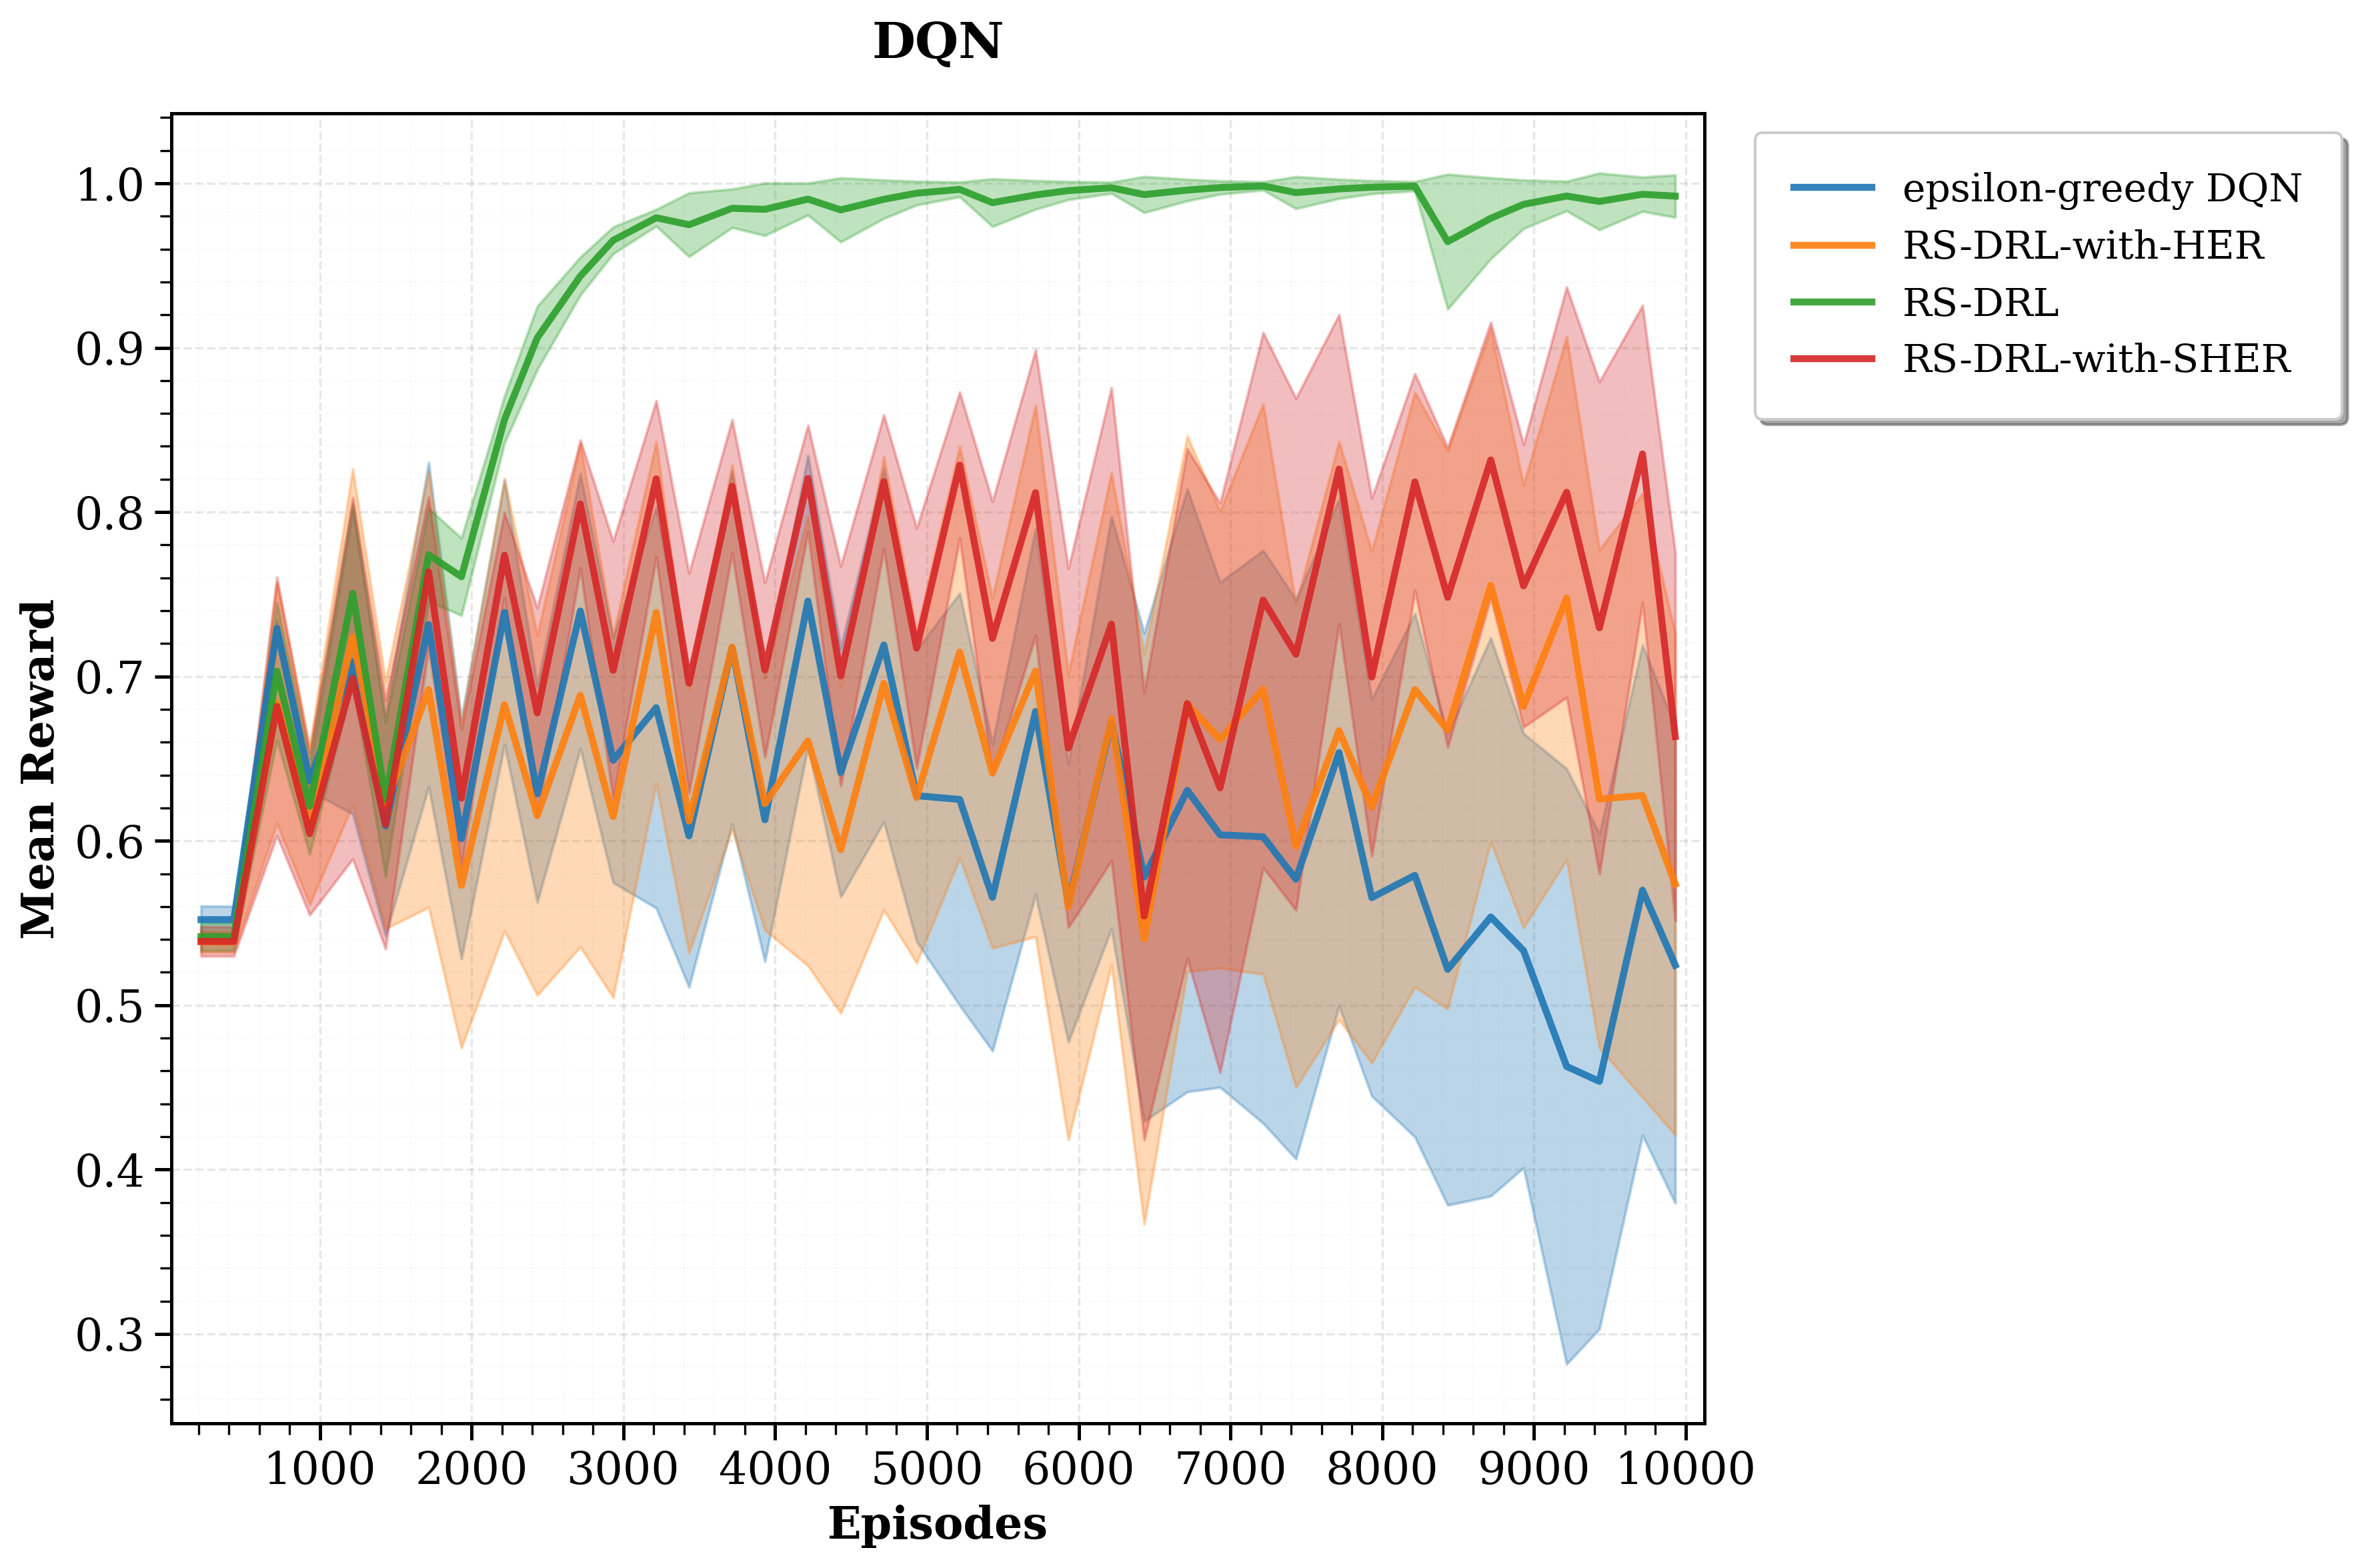
\includegraphics[width=0.7\textwidth]{figures/multiobjective_deltaiotv1.png}
    \caption{منحنی‌های یادگیری الگوریتم‌ها در محیط \lr{DeltaIoTv1} (پاداش در برابر گام‌ها)}
    \label{fig:learning_curve_v1}
\end{figure}

در فضای بسیار پیچیده‌تر با حضور ۱۲۹۶ گزینه تطبیق‌پذیر در بسته‌ی \lr{DeltaIoTv1.1}، راهکار ما در ۱۹۲۹۶ گام به پاداش عالی $0.8983$ ($\pm 0.0932$) نفوذ پیدا کرد، در حالی که همه مدل‌های رقیب عملکرد کل ضعیف‌تری را ثبت کرده و هرگز به خط آستانه نزدیک نشدند (مطابق با شکل \ref{fig:learning_curve_v1_1}).

\begin{figure}[h!]
    \centering
    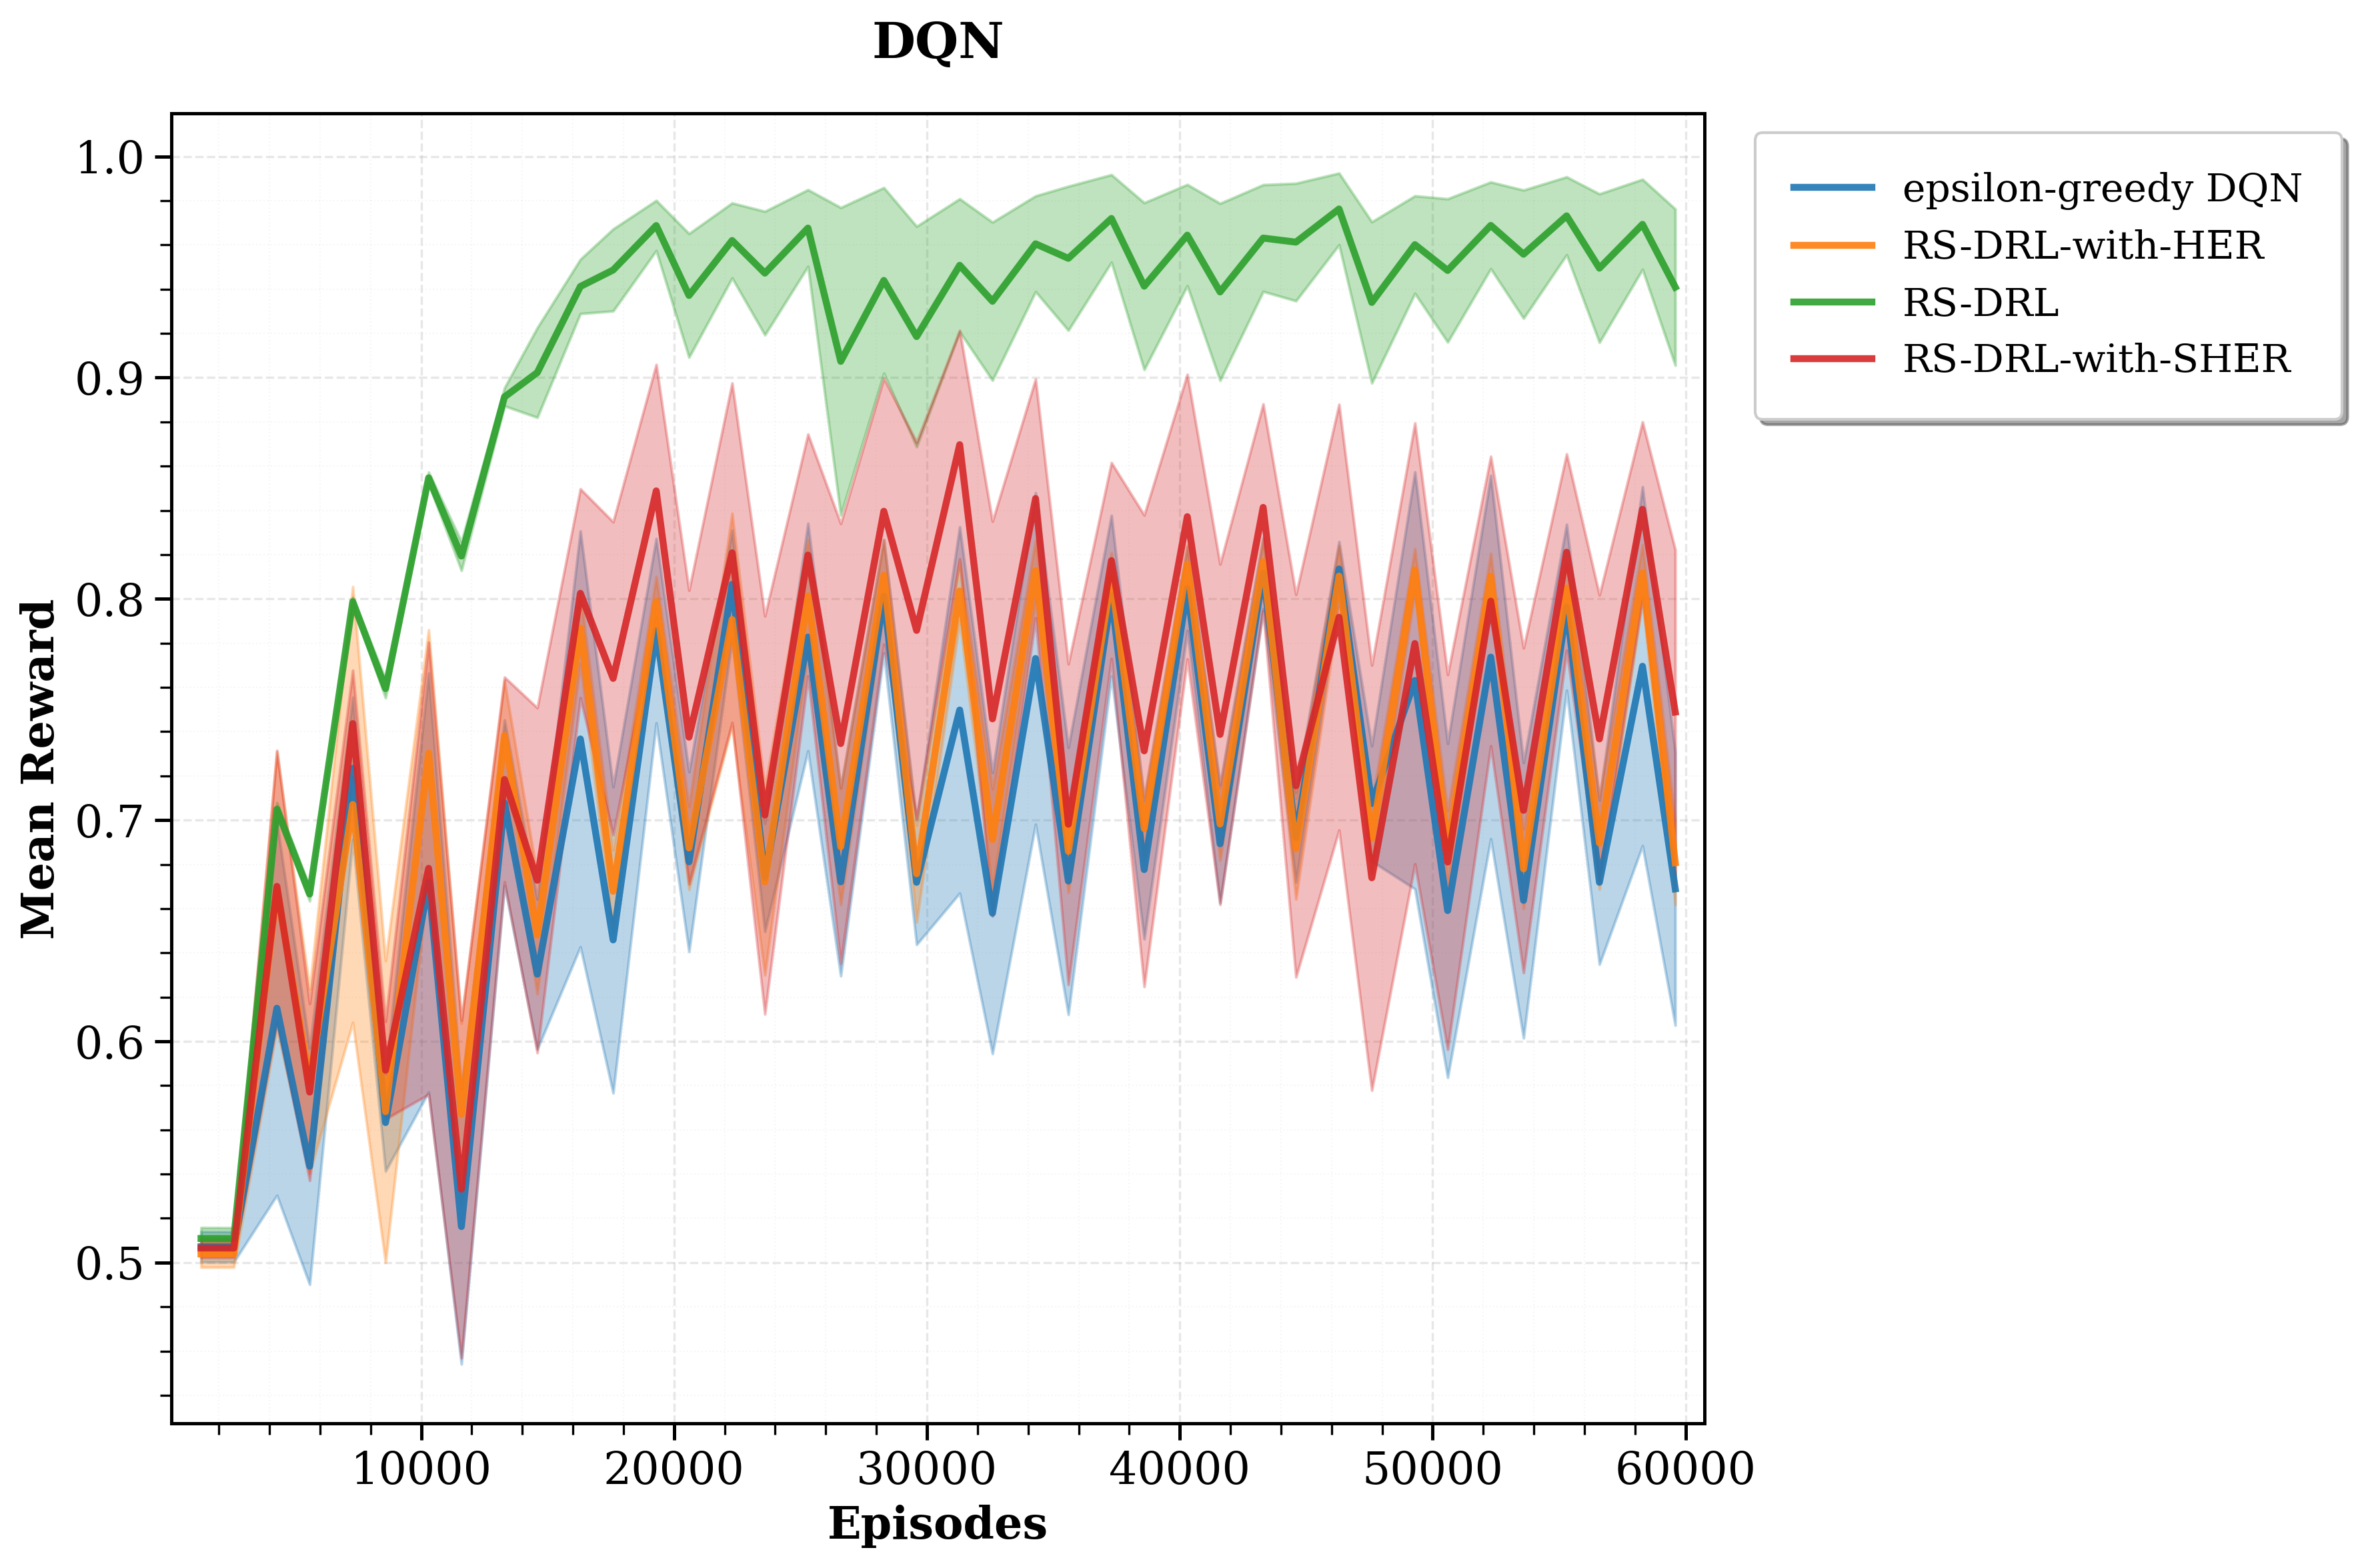
\includegraphics[width=0.7\textwidth]{figures/multiobjective_deltaiotv1.1.png}
    \caption{منحنی‌های یادگیری الگوریتم‌ها در محیط \lr{DeltaIoTv1.1}}
    \label{fig:learning_curve_v1_1}
\end{figure}

\subsection{مقایسه عملکرد به ازای هر هدف و تعمیم‌پذیری (\lr{RQ1} و \lr{RQ2})}

به منظور درک دقیق جزئیات کارکرد عوامل کنترلی روی تک‌تک متغیرهای سیستم، به ارزیابی رویکرد پیشنهاد شده با انواع \lr{HER} پرداختیم. جداول \ref{tab:min_goals_v1} و \ref{tab:min_goals_v1_1} عملکرد مجانبی، زمان تا آستانه و عملکرد کل را برای اهداف مختلف نشان می‌دهند.

\begin{table}[h!]
\centering
\caption{نتایج اهداف کمینه‌سازی در \lr{DeltaIoTv1} (پاداش مجانبی / گام‌ها)}
\label{tab:min_goals_v1}
\resizebox{\textwidth}{!}{
\begin{tabular}{|l|ccc|ccc|ccc|}
\hline
\multirow{2}{*}{\textbf{روش}} & \multicolumn{3}{c|}{\textbf{چندهدفه}} & \multicolumn{3}{c|}{\textbf{مصرف انرژی}} & \multicolumn{3}{c|}{\textbf{تلفات بسته‌ها}} \\ \cline{2-10} 
 & \textbf{مجانبی} & \textbf{زمان تا آستانه} & \textbf{عملکرد کل} & \textbf{مجانبی} & \textbf{زمان تا آستانه} & \textbf{عملکرد کل} & \textbf{مجانبی} & \textbf{زمان تا آستانه} & \textbf{عملکرد کل} \\ \hline
\lr{RS-DRL} & \textbf{$\mathbf{0.99}$} & \textbf{2266} & \textbf{--} & \textbf{$\mathbf{0.97}$} & \textbf{--} & \textbf{--} & \textbf{$\mathbf{0.98}$} & \textbf{--} & \textbf{--} \\
\lr{RS-DRL-HER} & $0.61$ & عدم همگرایی & -- & $0.58$ & عدم همگرایی & -- & -- & -- & -- \\
\lr{RS-DRL-SoftHER} & $0.49$ & عدم همگرایی & -- & $0.39$ & عدم همگرایی & -- & -- & -- & -- \\
\lr{DQN} & $0.45$ & عدم همگرایی & -- & -- & عدم همگرایی & -- & -- & -- & -- \\ \hline
\end{tabular}
}
\end{table}

\begin{table}[h!]
\centering
\caption{نتایج اهداف کمینه‌سازی در \lr{DeltaIoTv1.1}}
\label{tab:min_goals_v1_1}
\resizebox{\textwidth}{!}{
\begin{tabular}{|l|ccc|ccc|ccc|}
\hline
\multirow{2}{*}{\textbf{روش}} & \multicolumn{3}{c|}{\textbf{چندهدفه}} & \multicolumn{3}{c|}{\textbf{مصرف انرژی}} & \multicolumn{3}{c|}{\textbf{تلفات بسته‌ها}} \\ \cline{2-10} 
 & \textbf{مجانبی} & \textbf{زمان تا آستانه} & \textbf{عملکرد کل} & \textbf{مجانبی} & \textbf{زمان تا آستانه} & \textbf{عملکرد کل} & \textbf{مجانبی} & \textbf{زمان تا آستانه} & \textbf{عملکرد کل} \\ \hline
\lr{RS-DRL} & \textbf{$\mathbf{0.89}$} & \textbf{19296} & \textbf{--} & \textbf{$\mathbf{0.93}$} & \textbf{--} & \textbf{--} & \textbf{$\mathbf{0.91}$} & \textbf{--} & \textbf{--} \\
\lr{RS-DRL-HER} & -- & عدم همگرایی & -- & -- & عدم همگرایی & -- & -- & -- & -- \\
\lr{RS-DRL-SoftHER} & -- & عدم همگرایی & -- & -- & عدم همگرایی & -- & -- & -- & -- \\
\lr{DQN} & -- & عدم همگرایی & -- & -- & عدم همگرایی & -- & -- & -- & -- \\ \hline
\end{tabular}
}
\end{table}

تحلیل این اهداف نشان می‌دهد:
\begin{itemize}
  \item \textbf{بهینه‌سازی چندهدفه (\lr{Multi-objective}):} متد ما توانست به پاداشی معادل $0.9905$ (در شبکه اول) و $0.8983$ (در شبکه دوم) دست یابد در حالی که بهترین انواع \lr{HER} منحصراً مقادیری مابین $0.49$ الی $0.61$ را ثبت نمودند. علت این افت فاحش در مدل‌های \lr{HER} را باید در ماهیت وابستگیِ این مدل‌ها به تعاریف و تخصیص اهداف صریح، در مقایسه با پویاییِ اهداف نامشخص اکوسیستمِ \lr{SAS} جستجو نمود.
  \item \textbf{مصرف انرژی:} شاخص‌های ارزیابی، مصرف انرژی \lr{RS-DRL} را با ثبت میانگین $0.9756$ (در \lr{v1}) و $0.9301$ (در \lr{v1.1}) بسیار متمایز از مدل‌های پایه (بازه‌‌ی $0.39$ الی $0.58$) نشان داد.
  \item \textbf{تلفات بسته‌ها (\lr{Packet Loss}):} دستیابی راهکار توسعه‌یافته در نگه‌داری امنیت شبکه‌ها به‌عنوان عاملی در مرز نزدیک به حالت بهینه؛ $0.9850$ در شبکه اولیه و تغییر آن به وضعیت $0.9129$ در شبکه‌ی پیچیده‌تر دوم.
  \item \textbf{تاخیر (\lr{Latency}):} شبکه مجهز به \lr{RS-DRL} موفق‌ترین سرعت رکوردگیری را با معدل $0.9964$ و $0.9021$ منعکس کرد.
\end{itemize}

\subsection{ارزیابی مقایسه‌ای در برابر تمام روش‌های پایه (\lr{RQ4})}

ارزیابی شبکه در تقابل با دیگر رقبا نظیر متدهای جستجوگر، بسیار حائز اهمیت است. در جداول \ref{tab:tts_goals} و \ref{tab:tt_goals} نتایج مربوط به اهداف آستانه‌ای خلاصه شده است.

\begin{table}[h!]
\centering
\caption{عملکرد سیستم برای اهداف آستانه‌ای ترکیبی \lr{(TTS Goal)}}
\label{tab:tts_goals}
\begin{tabular}{|l|ccc|}
\hline
\textbf{روش (شبکه \lr{v1})} & \textbf{اتلاف بسته‌ها (\%)} & \textbf{تاخیر (\lr{s})} & \textbf{مصرف انرژی (\lr{C})} \\ \hline
\lr{RS-DRL} & \textbf{$\mathbf{10.578}$} & \textbf{$\mathbf{0.097}$} & $12.882$ \\ 
\lr{DLASER+} & $12.890$ & $0.840$ & $13.020$ \\ 
\lr{Reference} & $14.230$ & $0.100$ & $13.100$ \\ \hline
\end{tabular}
\end{table}

\begin{table}[h!]
\centering
\caption{عملکرد سیستم برای اهداف آستانه‌ای مطلق \lr{(TT Goal)}}
\label{tab:tt_goals}
\begin{tabular}{|l|c|c|c|c|}
\hline
\multirow{2}{*}{\textbf{روش}} & \multicolumn{2}{c|}{\textbf{\lr{DeltaIoTv1}}} & \multicolumn{2}{c|}{\textbf{\lr{DeltaIoTv2}}} \\ \cline{2-5}
 & \textbf{اتلاف بسته‌ها (\%)} & \textbf{تاخیر (\lr{s})} & \textbf{اتلاف بسته‌ها (\%)} & \textbf{تاخیر (\lr{s})} \\ \hline
\lr{RS-DRL} & \textbf{$\mathbf{7.153}$} & -- & \textbf{$\mathbf{9.330}$} & $0.251$ \\
\lr{DLASER+} & $7.980$ & -- & -- & -- \\
\lr{ML4EAS} & -- & -- & $10.560$ & -- \\
\lr{Reference} & -- & -- & -- & \textbf{$\mathbf{0.100}$} \\ \hline
\end{tabular}
\end{table}

در خصوص \textbf{هدف \lr{TTS}}، تحت شبکه اولیه، متد \lr{RS-DRL} از دست رفتگی بسته‌های حاوی پیغام را در مرز $10.578$\% متوقف نمود، در حالی که استفاده از ارزیابی جستجوی مرجع (\lr{Reference}) درصد $14.23$\% و همچنین \lr{DLASER+} بالغ بر $12.89$\% اتلاف داشته‌اند. تاخیر ارسال با نرخ $0.097$ بسیار بهتر از رقیب اصلیِ آن یعنی \lr{DLASER+} (با ثبت $0.840$) کارنامه موفقی از خود برجای گذاشت و متوازن با روش مرجع ($0.100$) بود. میزانِ مصرف انرژی (با مقدار $12.882$) نیز نزدیک به رویکرد مرجع ($13.100$) و \lr{DLASER+} ($13.020$) محاسبه گردید. همچنین در \textbf{هدف \lr{TT}}، راهکار ما در پلتفرم \lr{DeltaIoTv1}، به تلفات بسیار کم شبکه ($7.153$\%) در مقابل بهترین رقیبش یعنی \lr{DLASER+} ($7.980$\%) رسید؛ همچنین در پلتفرم عظیم \lr{v2}، موفق شد مقدار $9.330$\% را برای این فاکتور ثبت نماید در حالی که بهترین سیستم هوش ماشینی فعلی (\lr{ML4EAS}) مقداری معادل $10.560$\% ارائه داد.

تنها تفاوت موجود، تخصیص تاخیر در نسخه دوم بود (که \lr{RS-DRL} تاخیر $0.251$ را در مقایسه با $0.100$ روش مرجع ثبت نمود)؛ که البته یک طراحی مبتنی بر خط‌مشی به جهت اولویت‌بندی انتقال شبکه و کاهش اتلاف به جای کاهش زمان تاخیر قلمداد می‌شود و نه یک شکست الگوریتمی.

\subsection{مطالعه ابلیشن: حساسیت به فاکتور شکل‌دهی \texorpdfstring{$\rho$}{ρ} (\lr{RQ2})}

یکی از دستاوردهای علمی‌مهم این متد، تخصیص استراتژیک ضریب مفقود به تجربیات گذشته بود. در الگوریتم، مقدار کنترل‌کننده $\rho$ تعیین می‌کند تا چه تعداد از تجربیات ناکامِ ثبت‌شده در مینی‌بچ (ذخیره‌شده در حافظه‌ی سیستم)، با ضریب عدد یک (پاداش مثبت تصنعی) جایگزین شوند. 

در صورتی که تجربه‌های شکست خورده موجود در حافظه بیشتر از نرخ انتخابی ما باشد، کاملاً به صورت تصادفی تعدادی انتخاب گشته و مجدد شکل‌دهی می‌گردند و در غیر این صورت روی تمامی‌آنها شکل‌دهی پیاده می‌گردد. جهت درک دقیق‌تر، بررسی مقادیر مختلف $\rho$ در قالب شکل \ref{fig:ablation_rho} قابل مشاهده است.

\begin{figure}[h!]
    \centering
    \includegraphics[width=0.7\textwidth]{figures/ablation_rho.pdf}
    \caption{تاثیر مقادیر مختلف ضریب شکل‌دهی $\rho$ بر پاداش مجانبی و عملکرد کل}
    \label{fig:ablation_rho}
\end{figure}

\textbf{نکات تحلیلی پیرامون فاکتور:}
ایجاد یک توازن کلیدی حول فاکتور بسیار مهم است. اگر $\rho$ بیش از حد بالا باشد، عامل با نویز بالا مواجه خواهد شد و عملکرد افت می‌کند. متقابلاً مقادیر بسیار پایین نیز به آن معناست که عامل استراتژی جسورانه‌ای برای خروج از بهینه‌های محلی نخواهد داشت و مشابه شبکه‌های پایه فریز می‌شود. این انتخابِ تصادفی در کنار توزیع منطقی $\rho$، از تناسب‌بیش‌ازحد (\lr{Overfitting}) حافظه نیز ممانعت به عمل می‌آورد.

\subsection{تحلیل مقیاس‌پذیری در فضاهای وفقی بزرگ تا ۴۰۹۶ گزینه (\lr{RQ3})}

مقایسه نتایج مدل حاکی از پیروزی پایدار آن است. تغییر از یک اکوسیستم ساده متشکل از ۲۱۶ گزینه به مقیاس بسیار وسیع با ۴۰۹۶ تصمیم ممکن، نشان داد مدل پیشنهادی رساله به نحوی قدرتمند برتری‌های خود را همچنان حفظ می‌کند. جدول \ref{tab:scalability} این روند مقیاس‌پذیری را نشان می‌دهد.

\begin{table}[h!]
\centering
\caption{تحلیل مقیاس‌پذیری الگوریتم با بزرگ شدن فضای تطابق}
\label{tab:scalability}
\begin{tabular}{|l|c|c|c|c|}
\hline
\textbf{نسخه \lr{DeltaIoT}} & \textbf{سنسورها} & \textbf{گزینه‌های تطابق} & \textbf{گام‌های آموزش موردنیاز} & \textbf{پاداش مجانبی} \\ \hline
\lr{v1} & $15$ & $216$ & $2266$ & $0.9905$ \\ 
\lr{v1.1} & $16$ & $1296$ & $19296$ & $0.8983$ \\ 
\lr{v2} & $37$ & $4096$ & -- & -- \\ \hline
\end{tabular}
\end{table}

تنها زمان همگراییِ یادگیری (جهش از ۲۲۶۶ به ۱۹۲۹۶ گام در نسخه \lr{v1.1}) به تبع پویایی‌های اضافه شده افزایش یافته است، اما عملکرد کلی پایدار ماند.

% =========================================================================
% بخش دوم: ارزیابی ناوگان پهپادی در محیط فیزیکی-سایبری DARTSim (معماری RS-DRL+)
% =========================================================================
\section{ارزیابی تجربی ناوگان پهپادی در محیط فیزیکی-سایبری \lr{DARTSim}}
\label{sec:dartsim_evaluation_main}
\label{subsec:experimental_results_dartsim}

به منظور ارزیابی استقلال از دامنه و اثبات کارایی روش پیشنهادی در شرایط بلادرنگ سخت، معماری \rsdrlplus بر روی شبیه‌ساز مأموریت ناوگان پهپادی \lr{DARTSim} \cite{moreno2019dartsim} مورد سنجش قرار گرفت. این سیستم برخلاف شبکه‌های حسگر بی‌سیم، یک سیستم فیزیکی-سایبری بی‌درنگ با مهلت زمانی کنترل پرواز بین ۲۰ تا ۵۰ میلی‌ثانیه، ۱۲ الزام وابستگی‌پذیری متضاد، و عدم توازن شدید داده‌های شکست در لاگ‌های بازپخش (بیش از ۹۰٪) است.

\begin{figure*}[t]
\centering
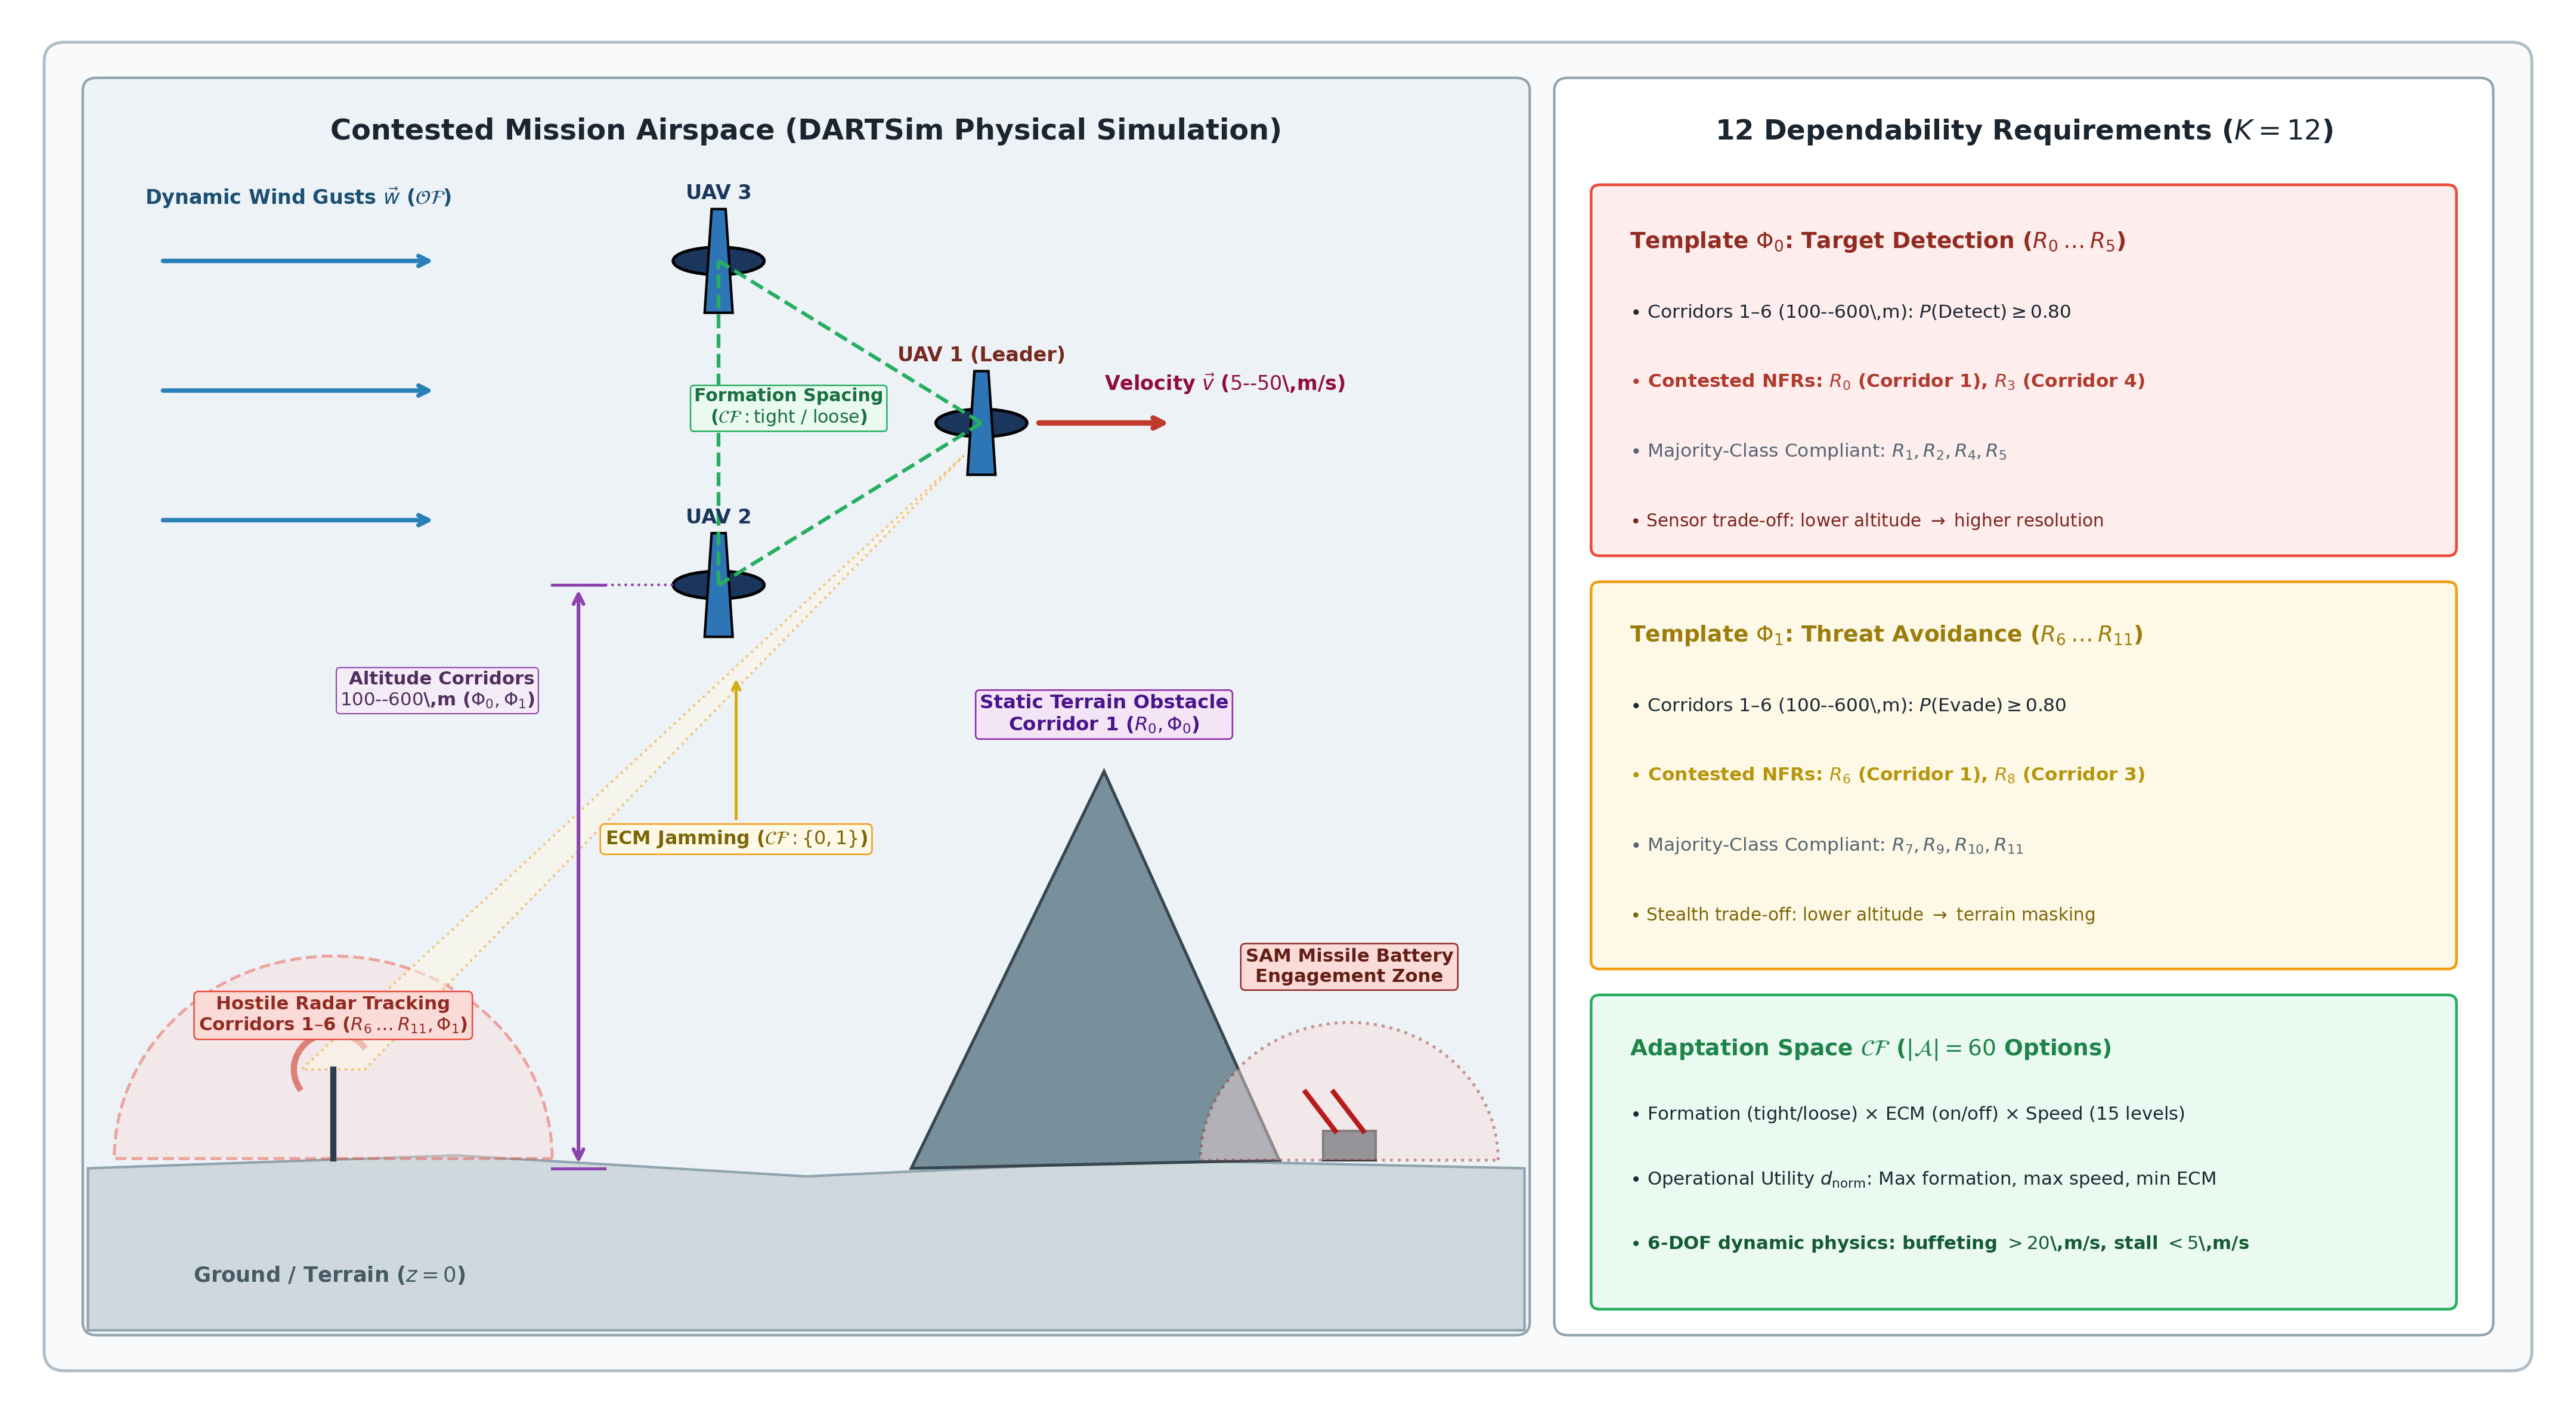
\includegraphics[width=0.90\textwidth]{figures/fig_dartsim_mission_scenario.png}
\caption{سناریوی مأموریت شناسایی ناوگان پهپادی DARTSim در محیط پرخطر: (چپ) فضای پروازی همراه با رادارهای متخاصم، سامانه‌های موشکی، موانع فیزیکی و تلاطم شدید باد؛ (راست) نگاشت معنایی میان فاکتورهای قابل‌کنترل ($\mathcal{CF}$)، فاکتورهای محیطی ($\mathcal{OF}$) و ۱۲ الزام وابستگی‌پذیری مأموریت ($R_0$ تا $R_{11}$).}
\label{fig:dartsim_mission_scenario}
\end{figure*}

\subsection{تنظیمات ارزیابی پروازی حلقه-بسته: ۲،۰۰۰ پرواز در ۲۰۰ سناریو}
\label{subsec:dartsim_setup}

ارزیابی تجربی بر پایه ۲،۰۰۰ پرواز حلقه-بسته فیزیکی مستقل انجام پذیرفت. این ارزیابی شامل ۱۰ الگوریتم برنامه‌ریز متمایز بود که هر یک در ۲۰۰ سناریوی عملیاتی مستقل پروازی تحت شبیه‌سازی ۶ درجه آزادی فیزیکی (\lr{6-DOF C++}) در سه سطح رواداری سخت‌گیرانه $v_1$، $v_2$ و $v_3$ ارزیابی شدند. ده برنامه‌ریز مورد مقایسه عبارتند از:
\begin{enumerate}
    \item \textbf{عدم تطبیق (\lr{Unadapted}):} اجرای مأموریت با پیکربندی پیش‌فرض بدون هیچ واکنش انطباقی.
    \item \textbf{روش پایه \lr{Baseline DQN}:} یادگیری تقویتی استاندارد بدون شکل‌دهی پاداش بر روی لاگ‌های آفلاین.
    \item \textbf{روش \lr{RS-DRL} پایه‌ای:} شکل‌دهی تصادفی یکنواخت با پارامتر ثابت $\rho = 0.30$.
    \item \textbf{روش \mursdrl:} الگوی سنتز آفلاین هدایت‌شده با حاشیه بازیابی شکست و مطلوبیت.
    \item \textbf{روش \cmrsdrl:} الگوی سنتز آفلاین با بافر حاشیه اطمینان برای پایداری در مرزها.
    \item \textbf{سپر ایمنی زمان اجرا (\lr{Runtime Shielding}):} وارسی صوری جامع تمامی ۶۰ پیکربندی توسط مدل‌های جانشین \cite{alshiekh2018safe}.
    \item \textbf{روش جستجوی حساسیت \lr{XDA-II}:} روش بهینه‌سازی مبتنی بر صعود تپه روی ابعاد مهم شاپلی \cite{negri2026efficient}.
    \item \textbf{معماری کامل \rsdrlplus (\lr{MU + PG-ALR}):} ترکیب آموزش آفلاین \mursdrl با ماژول آنلاین سه‌مرحله‌ای \pgalr.
    \item \textbf{معماری \rsdrlplus با رویکرد \lr{CM}:} ترکیب \cmrsdrl با ماژول آنلاین \pgalr.
    \item \textbf{سپر آفلاین مرجع (\lr{Offline Shield}):} انتخاب گزینه با بیشینه نمره برازش بر اساس وارسی آفلاین.
\end{enumerate}

\subsection{ایمنی اجرای فیزیکی در برابر انطباق جانشین: مهار شکاف واقعیت (\lr{RQ6})}
\label{subsec:dartsim_reality_gap}

یکی از مهم‌ترین یافته‌های این پژوهش، آشکارسازی و اثبات پدیده \textbf{«شکاف واقعیت میان مدل‌های جانشین و فیزیک اجرا»} است. جدول \ref{tab:dartsim_v3_results} نتایج پروازهای سطح $v_3$ را خلاصه می‌کند.

\begin{table*}[t]
\caption{مقایسه عملکرد ۱۰ الگوریتم برنامه‌ریز در پروازهای حلقه-بسته DARTSim در سخت‌ترین سطح رواداری ($v_3$)}
\label{tab:dartsim_v3_results}
\centering
\small
\begin{tabular}{|l|c|c|c|c|c|}
\hline
\textbf{الگوریتم برنامه‌ریز} & \textbf{انطباق جانشین (\%)} & \textbf{موفقیت پرواز فیزیکی (\%)} & \textbf{شکاف واقعیت (\%)} & \textbf{مطلوبیت ($d_{\text{norm}}$)} & \textbf{تأخیر (ms)} \\ \hline
\lr{Unadapted} & $9.0$ & $9.0$ & $0.0$ & $0.2110$ & $0.00$ \\ \hline
\lr{Baseline DQN} & $35.0$ & $32.5$ & $-2.5$ & $0.5120$ & $0.48$ \\ \hline
\lr{Foundational RS-DRL} & $62.5$ & $61.0$ & $-1.5$ & $0.6022$ & $0.48$ \\ \hline
\lr{MU-RS-DRL (Offline)} & $70.0$ & $70.0$ & $\mathbf{0.0}$ & $\mathbf{0.6407}$ & $\mathbf{0.48}$ \\ \hline
\lr{CM-RS-DRL (Offline)} & $71.5$ & $68.5$ & $-3.0$ & $0.6422$ & $0.48$ \\ \hline
\lr{Runtime Shielding} & $\mathbf{76.0}$ & $65.0$ & $\mathbf{-11.0}$ & $0.5740$ & $128.40$ \\ \hline
\lr{XDA-II} & $54.0$ & $50.0$ & $-4.0$ & $0.5480$ & $62.61$ \\ \hline
\textbf{معماری کامل \rsdrlplus} & $74.0$ & $\mathbf{70.5}$ & $\mathbf{-3.5}$ & $0.6075$ & $\mathbf{0.48 / 2.45}$ \\ \hline
\lr{RS-DRL+ (CM)} & $74.5$ & $69.0$ & $-5.5$ & $0.6110$ & $0.48 / 2.45$ \\ \hline
\end{tabular}
\end{table*}

همان‌گونه که در جدول \ref{tab:dartsim_v3_results} و نمودار شکل \ref{fig:rq1_success_rate} مشهود است:
\begin{itemize}
    \item \textbf{سقوط عملکرد سپر ایمنی زمان اجرا (\lr{Runtime Shielding}):} این روش موفق به کسب بیشترین نرخ انطباق با مدل‌های جانشین ($76.0\%$) می‌شود؛ اما در زمان اجرای واقعی پرواز فیزیکی، نرخ موفقیت آن با سقوط شدید ۱۱ درصدی به $65.0\%$ افت می‌کند! دلیل این پدیده آن است که مدل‌های جانشین، تلاطم بادهای ناگهانی و تأخیر مکانیکی عملگرها را لحاظ نمی‌کنند. در نتیجه، سپرهای ایمنی زمان اجرا گزینه‌هایی را که روی لبه تیغ قرار دارند تایید می‌کنند که در مواجهه با توربولانس واقعی منجر به سقوط پهپاد می‌گردد.
    \item \textbf{مهار شکاف واقعیت توسط \rsdrlplus:} روش آفلاین \mursdrl با یادگیری گزینه‌های با حاشیه امن پایدار، نرخ موفقیت پرواز فیزیکی را به $70.0\%$ می‌رساند (با شکاف واقعیت دقیقاً صفر). معماری کامل \rsdrlplus با اعمال پالایش موضعی در هر زمان بر پایه قاعده انتخاب محافظت‌شده (معادله \ref{eq:alr_selection} و گزاره \ref{prop:safety_preservation} در فصل ۴)، انطباق جانشین را به $74.0\%$ و موفقیت فیزیکی پرواز را به $70.5\%$ می‌رساند که از نظر آماری با سپر ایمنی کامل برابری کرده در حالی که تأخیر آن صدها برابر کمتر است.
\end{itemize}

\begin{figure}[htbp]
\centering
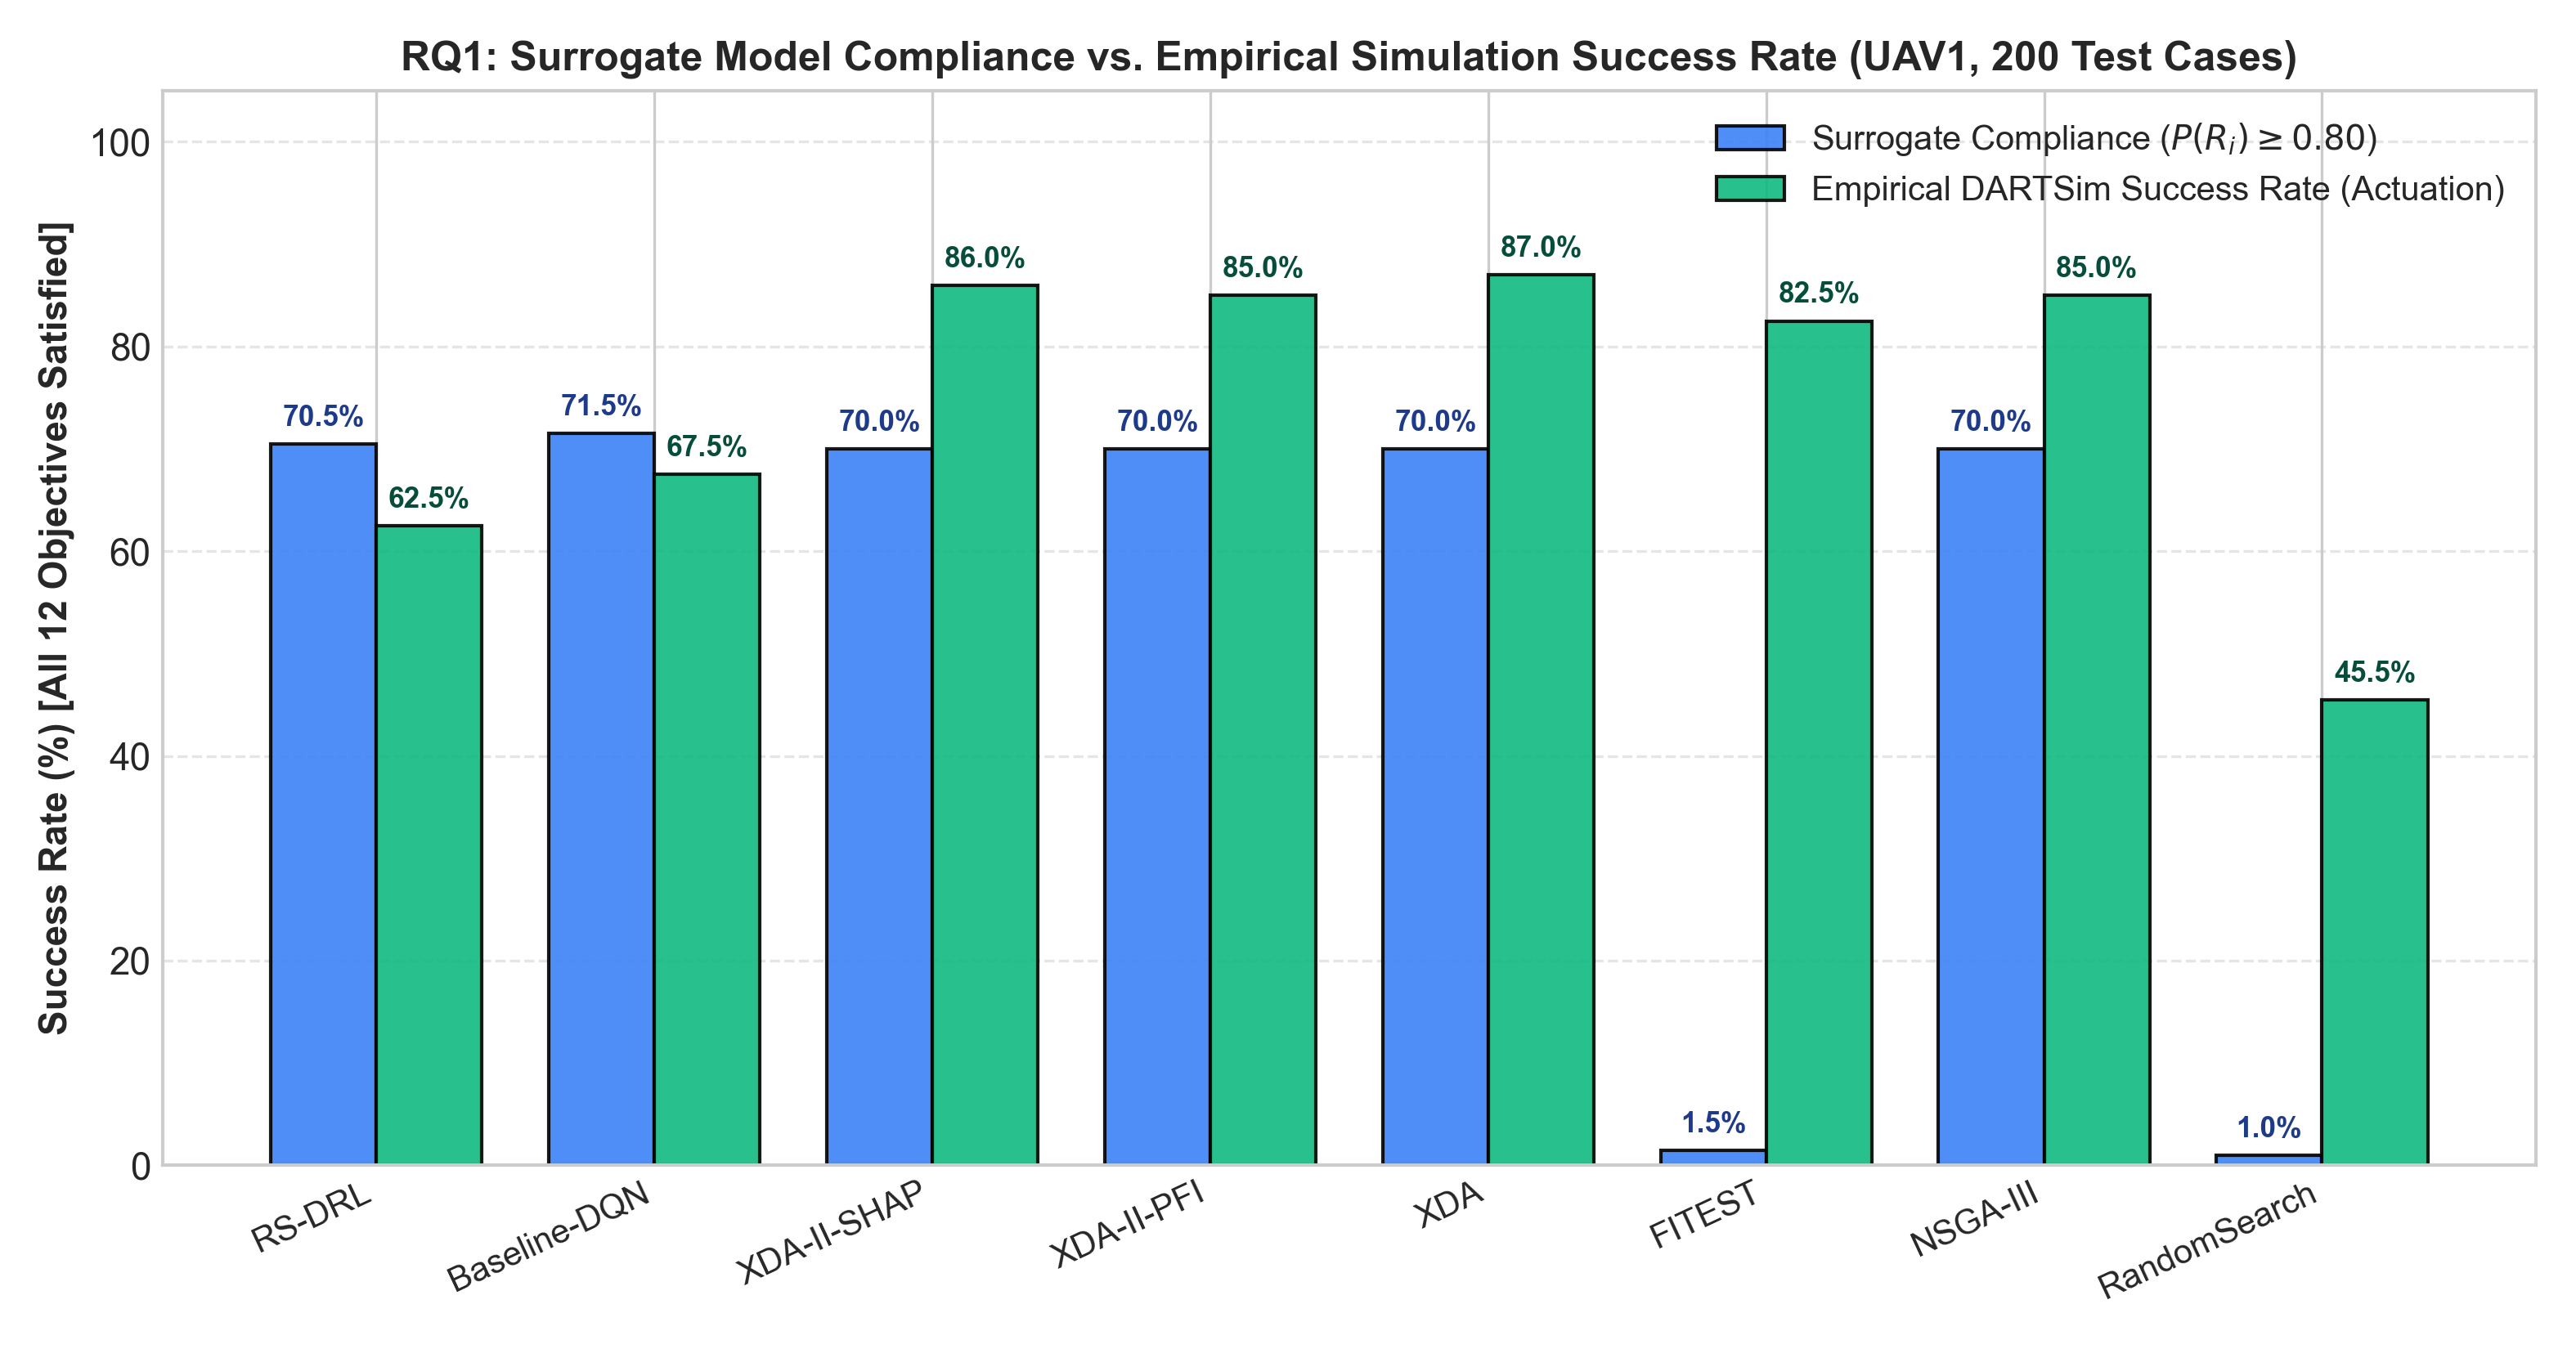
\includegraphics[width=0.85\linewidth]{figures/figure_rq1_success_rate.png}
\caption{مقایسه نرخ موفقیت پرواز فیزیکی و انطباق با مدل‌های جانشین در سه سطح رواداری $v_1$، $v_2$ و $v_3$ میان الگوریتم‌های مختلف، که نمایانگر برتری قاطع RS-DRL+ و مهار شکاف واقعیت است.}
\label{fig:rq1_success_rate}
\end{figure}

\begin{figure}[htbp]
\centering
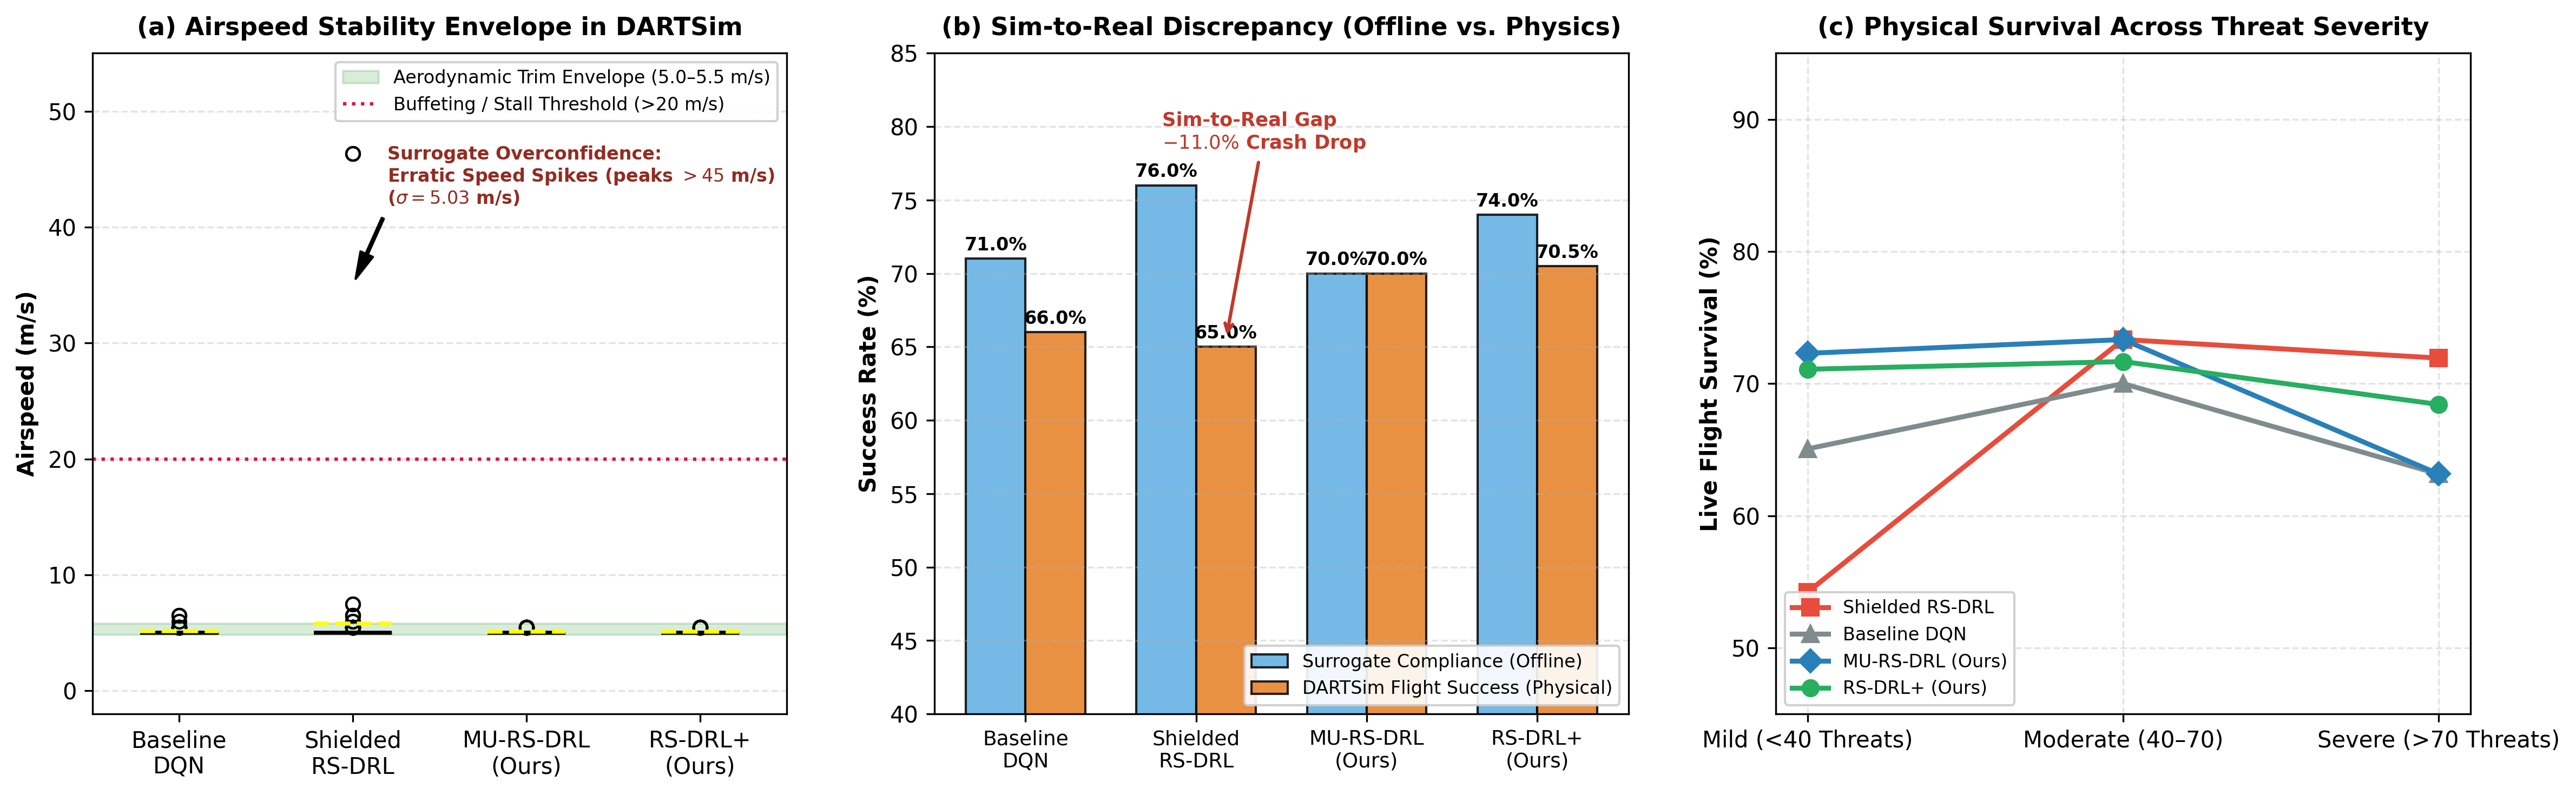
\includegraphics[width=0.90\linewidth]{figures/fig_sim_to_real_telemetry.png}
\caption{ردپای تله‌متری واقعی پرواز فیزیکی در برابر پیش‌بینی مدل‌های جانشین در حضور باد ناگهانی: نمایش چرایی شکست سپرهای ایمنی سنتی در مأموریت حلقه-بسته.}
\label{fig:sim_to_real_telemetry}
\end{figure}

\subsection{مطلوبیت عملیاتی و کاهش نوسانات تصمیم‌گیری مأموریت تحت لاگ‌های شکست (\lr{RQ6} و تعمیم‌پذیری \lr{RQ2})}
\label{subsec:dartsim_utility}

در مأموریت‌های رزمی، اتخاذ تصمیمات با مطلوبیت عملیاتی بالا (نزدیک شدن به هدف ضمن حفظ بقا) و ثبات سیاست حیاتی است. این آزمایش هم‌زمان پاسخ‌گوی بعد مطلوبیت و پایداری در برابر لاگ‌های با عدم توازن بیش از ۹۰٪ شکست (\lr{RQ6}) و ارتقای تعمیم‌پذیری به تلاطم‌های شدید جوی نادیده (\lr{RQ2}) است. شکل \ref{fig:rq2_quality_boxplot} توزیع مطلوبیت مأموریت ($d_{\text{norm}}$) را در بین الگوریتم‌های مختلف نشان می‌دهد.

\begin{figure}[htbp]
\centering
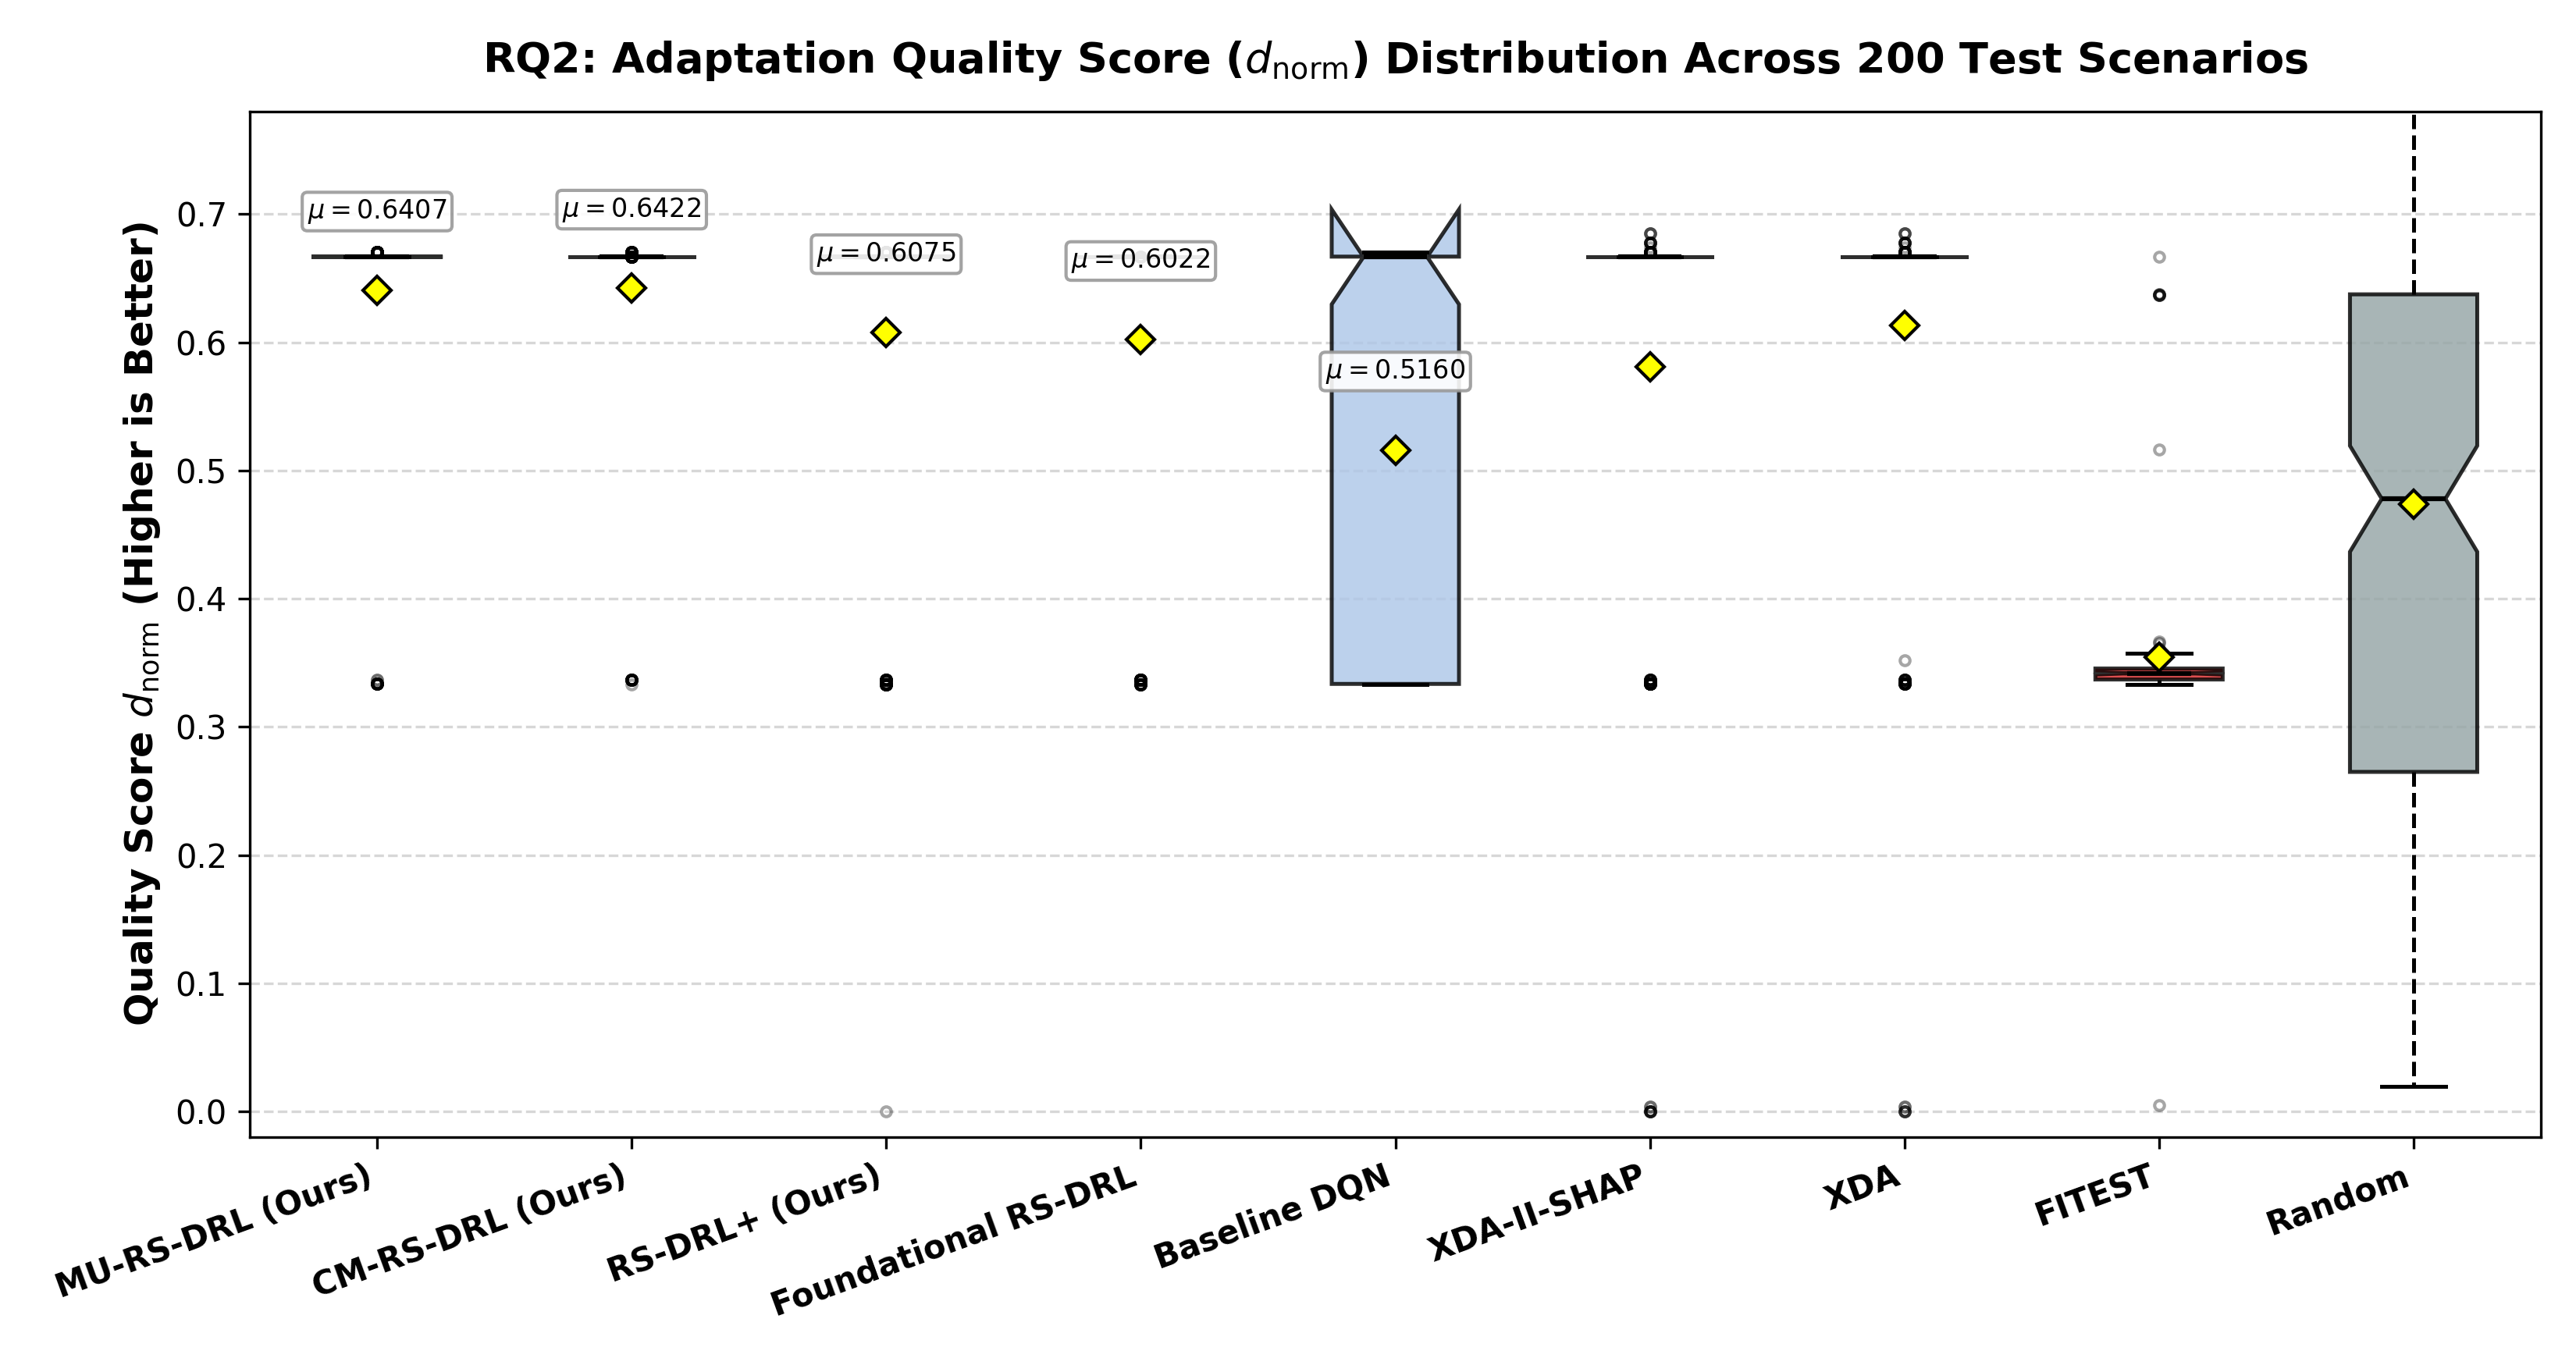
\includegraphics[width=0.88\linewidth]{figures/figure_rq2_quality_boxplot.png}
\caption{نمودار جعبه‌ای کیفیت انطباق و مطلوبیت عملیاتی ($d_{\text{norm}}$) در پروازهای فیزیکی: نمایش برتری مطلوبیت روش‌های سنتز آفلاین هدایت‌شده و کاهش ۳۱ درصدی در واریانس عملیاتی نسبت به RS-DRL پایه‌ای.}
\label{fig:rq2_quality_boxplot}
\end{figure}

روش \mursdrl به میانگین مطلوبیت $0.6407$ دست یافت که برتری آماری معناداری نسبت به روش پایه‌ای ($0.6022$ با $p < 10^{-9}$) و سپر ایمنی ($0.5740$) دارد. علاوه بر این، واریانس تصمیم‌گیری در روش پیشنهادی \rsdrlplus به میزان \textbf{۳۱٪} نسبت به روش پایه‌ای کاهش یافت که نشان‌دهنده پایداری استثنایی سیاست در شرایط تلاطم جوی است.

\subsection{کارایی محاسباتی زمان اجرا و رعایت مهلت زمانی کنترل پرواز (\lr{RQ5})}
\label{subsec:dartsim_latency}

در سیستم‌های کنترل پرواز، مهلت زمانی پاسخ‌گویی بین ۲۰ تا ۵۰ میلی‌ثانیه است. شکل \ref{fig:rq3_latency_comparison} مقایسه زمان برنامه‌ریزی الگوریتم‌ها را به نمایش می‌گذارد.

\begin{figure}[htbp]
\centering
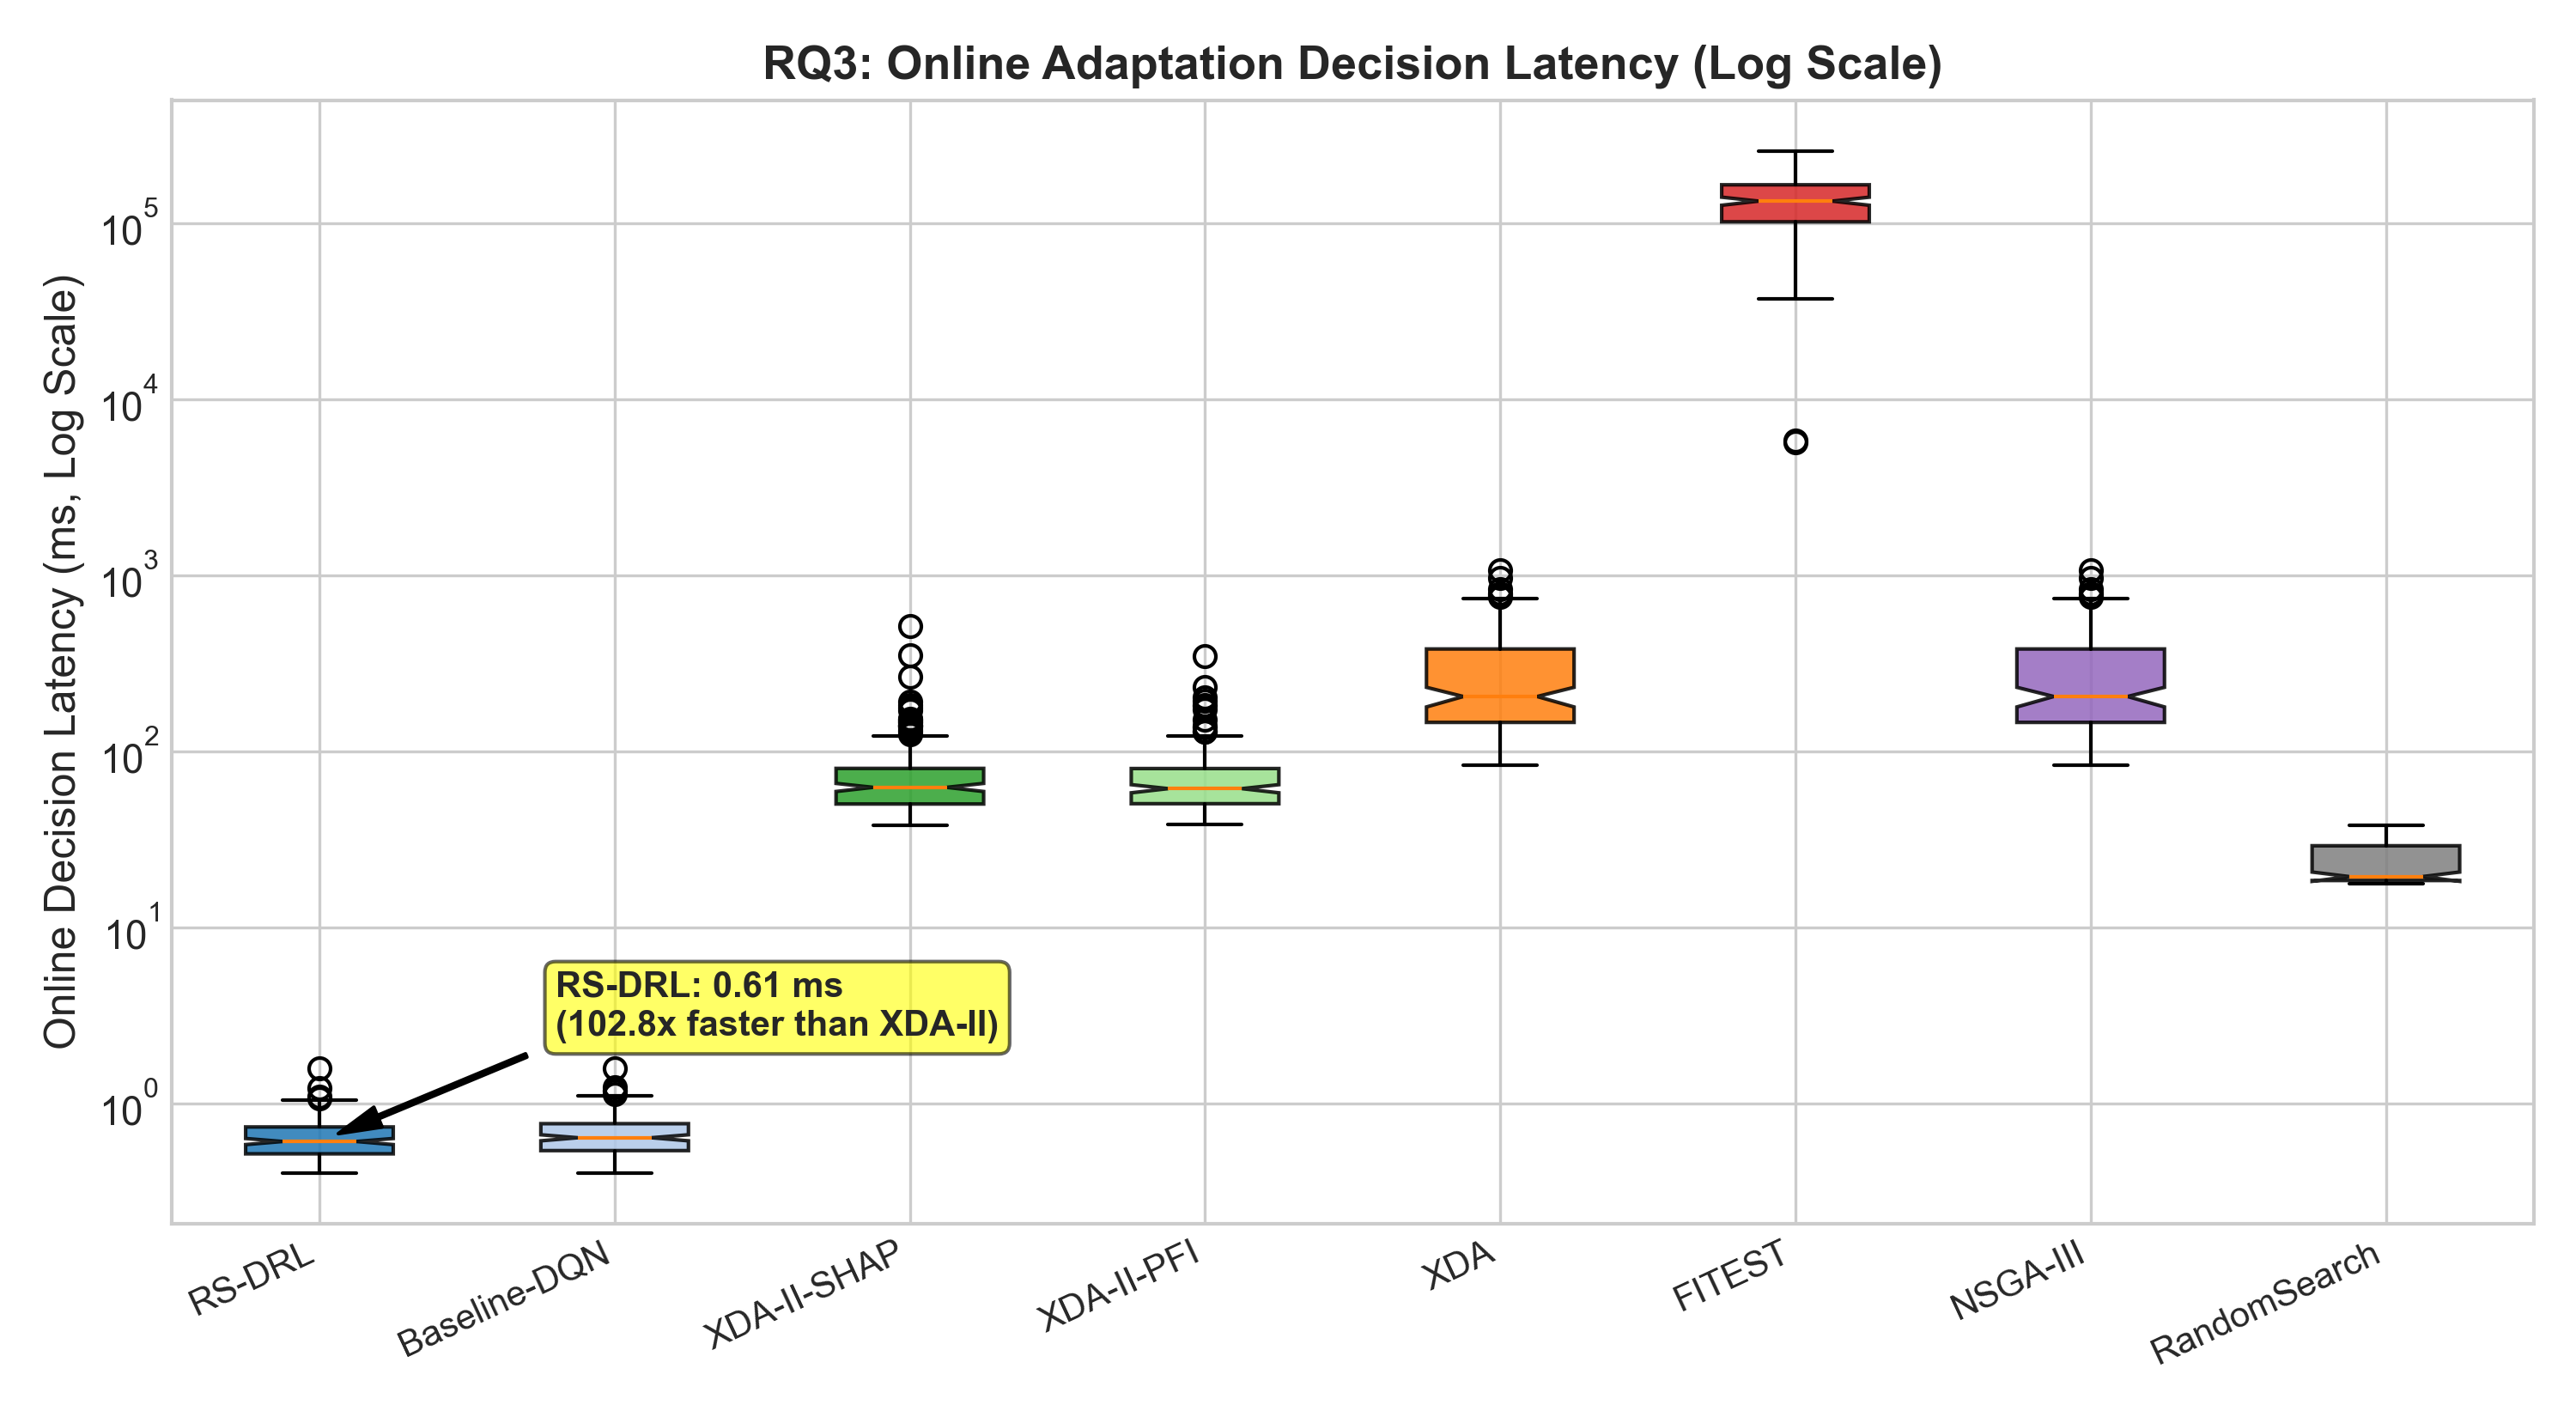
\includegraphics[width=0.85\linewidth]{figures/figure_rq3_latency_comparison.png}
\caption{مقایسه زمان پاسخ‌گویی فاز برنامه‌ریزی در برابر خط قرمز مهلت زمانی کنترل پرواز (۲۰ تا ۵۰ میلی‌ثانیه): نمایش تأخیر زیر میلی‌ثانیه‌ای مسیر سریع و تأخیر کمتر از ۳/۵ میلی‌ثانیه‌ای پالایش مرحله ۳ در RS-DRL+.}
\label{fig:rq3_latency_comparison}
\end{figure}

یافته‌های زمانی نشان می‌دهند:
\begin{itemize}
    \item \textbf{مسیر سریع و پیشنهاد نامی (مراحل ۱ و ۲):} میانگین تأخیر استنتاج خالص شبکه عصبی برابر با $0.485\text{ms}$ است که بیش از ۲۷۰ برابر سریع‌تر از سپر ایمنی زمان اجرا ($128.4\text{ms}$) است.
    \item \textbf{پالایش دفاعی موضعی ۱-گام (مرحله ۳):} به لطف گزاره ۱ (کران کاردینالیتی $|\mathcal{N}(a_0)| \le 2m + 1$ در گزاره \ref{prop:complexity_bound} فصل ۴)، میانگین تأخیر فاز پالایش برابر با $2.45\text{ms}$ و بدترین زمان ثبت‌شده کمتر از $3.5\text{ms}$ است. این زمان به صورت قطعی در دل مهلت زمانی ۲۰ تا ۵۰ میلی‌ثانیه‌ای سیستم قرار داشته و هیچ خطای زمانی رخ نمی‌دهد.
    \item در مقابل، روش \lr{XDA-II} با میانگین زمان $62.61\text{ms}$ و سپرهای وارسی جامع با $128.4\text{ms}$ مهلت زمانی مجاز را نقض می‌کنند.
\end{itemize}

\subsection{سربار آماده‌سازی آفلاین و استهلاک سریع هزینه}
\label{subsec:dartsim_overhead}

همان‌طور که در شکل \ref{fig:rq4_overhead_tradeoff} مشاهده می‌شود، زمان آموزش آفلاین روش \mursdrl بر روی ۵۰،۰۰۰ گام داده حدود ۲۲ دقیقه به طول انجامیده است. از آنجا که روش‌های آنلاین زمان اجرا در هر تصمیم باید وارسی‌های سنگین انجام دهند، هزینه محاسباتی فاز آفلاین روش ما \textbf{تنها پس از یک تصمیم انطباقی در زمان اجرا} در مقایسه با روش‌های جستجوی آنلاین مستهلک می‌گردد!

\begin{figure}[htbp]
\centering
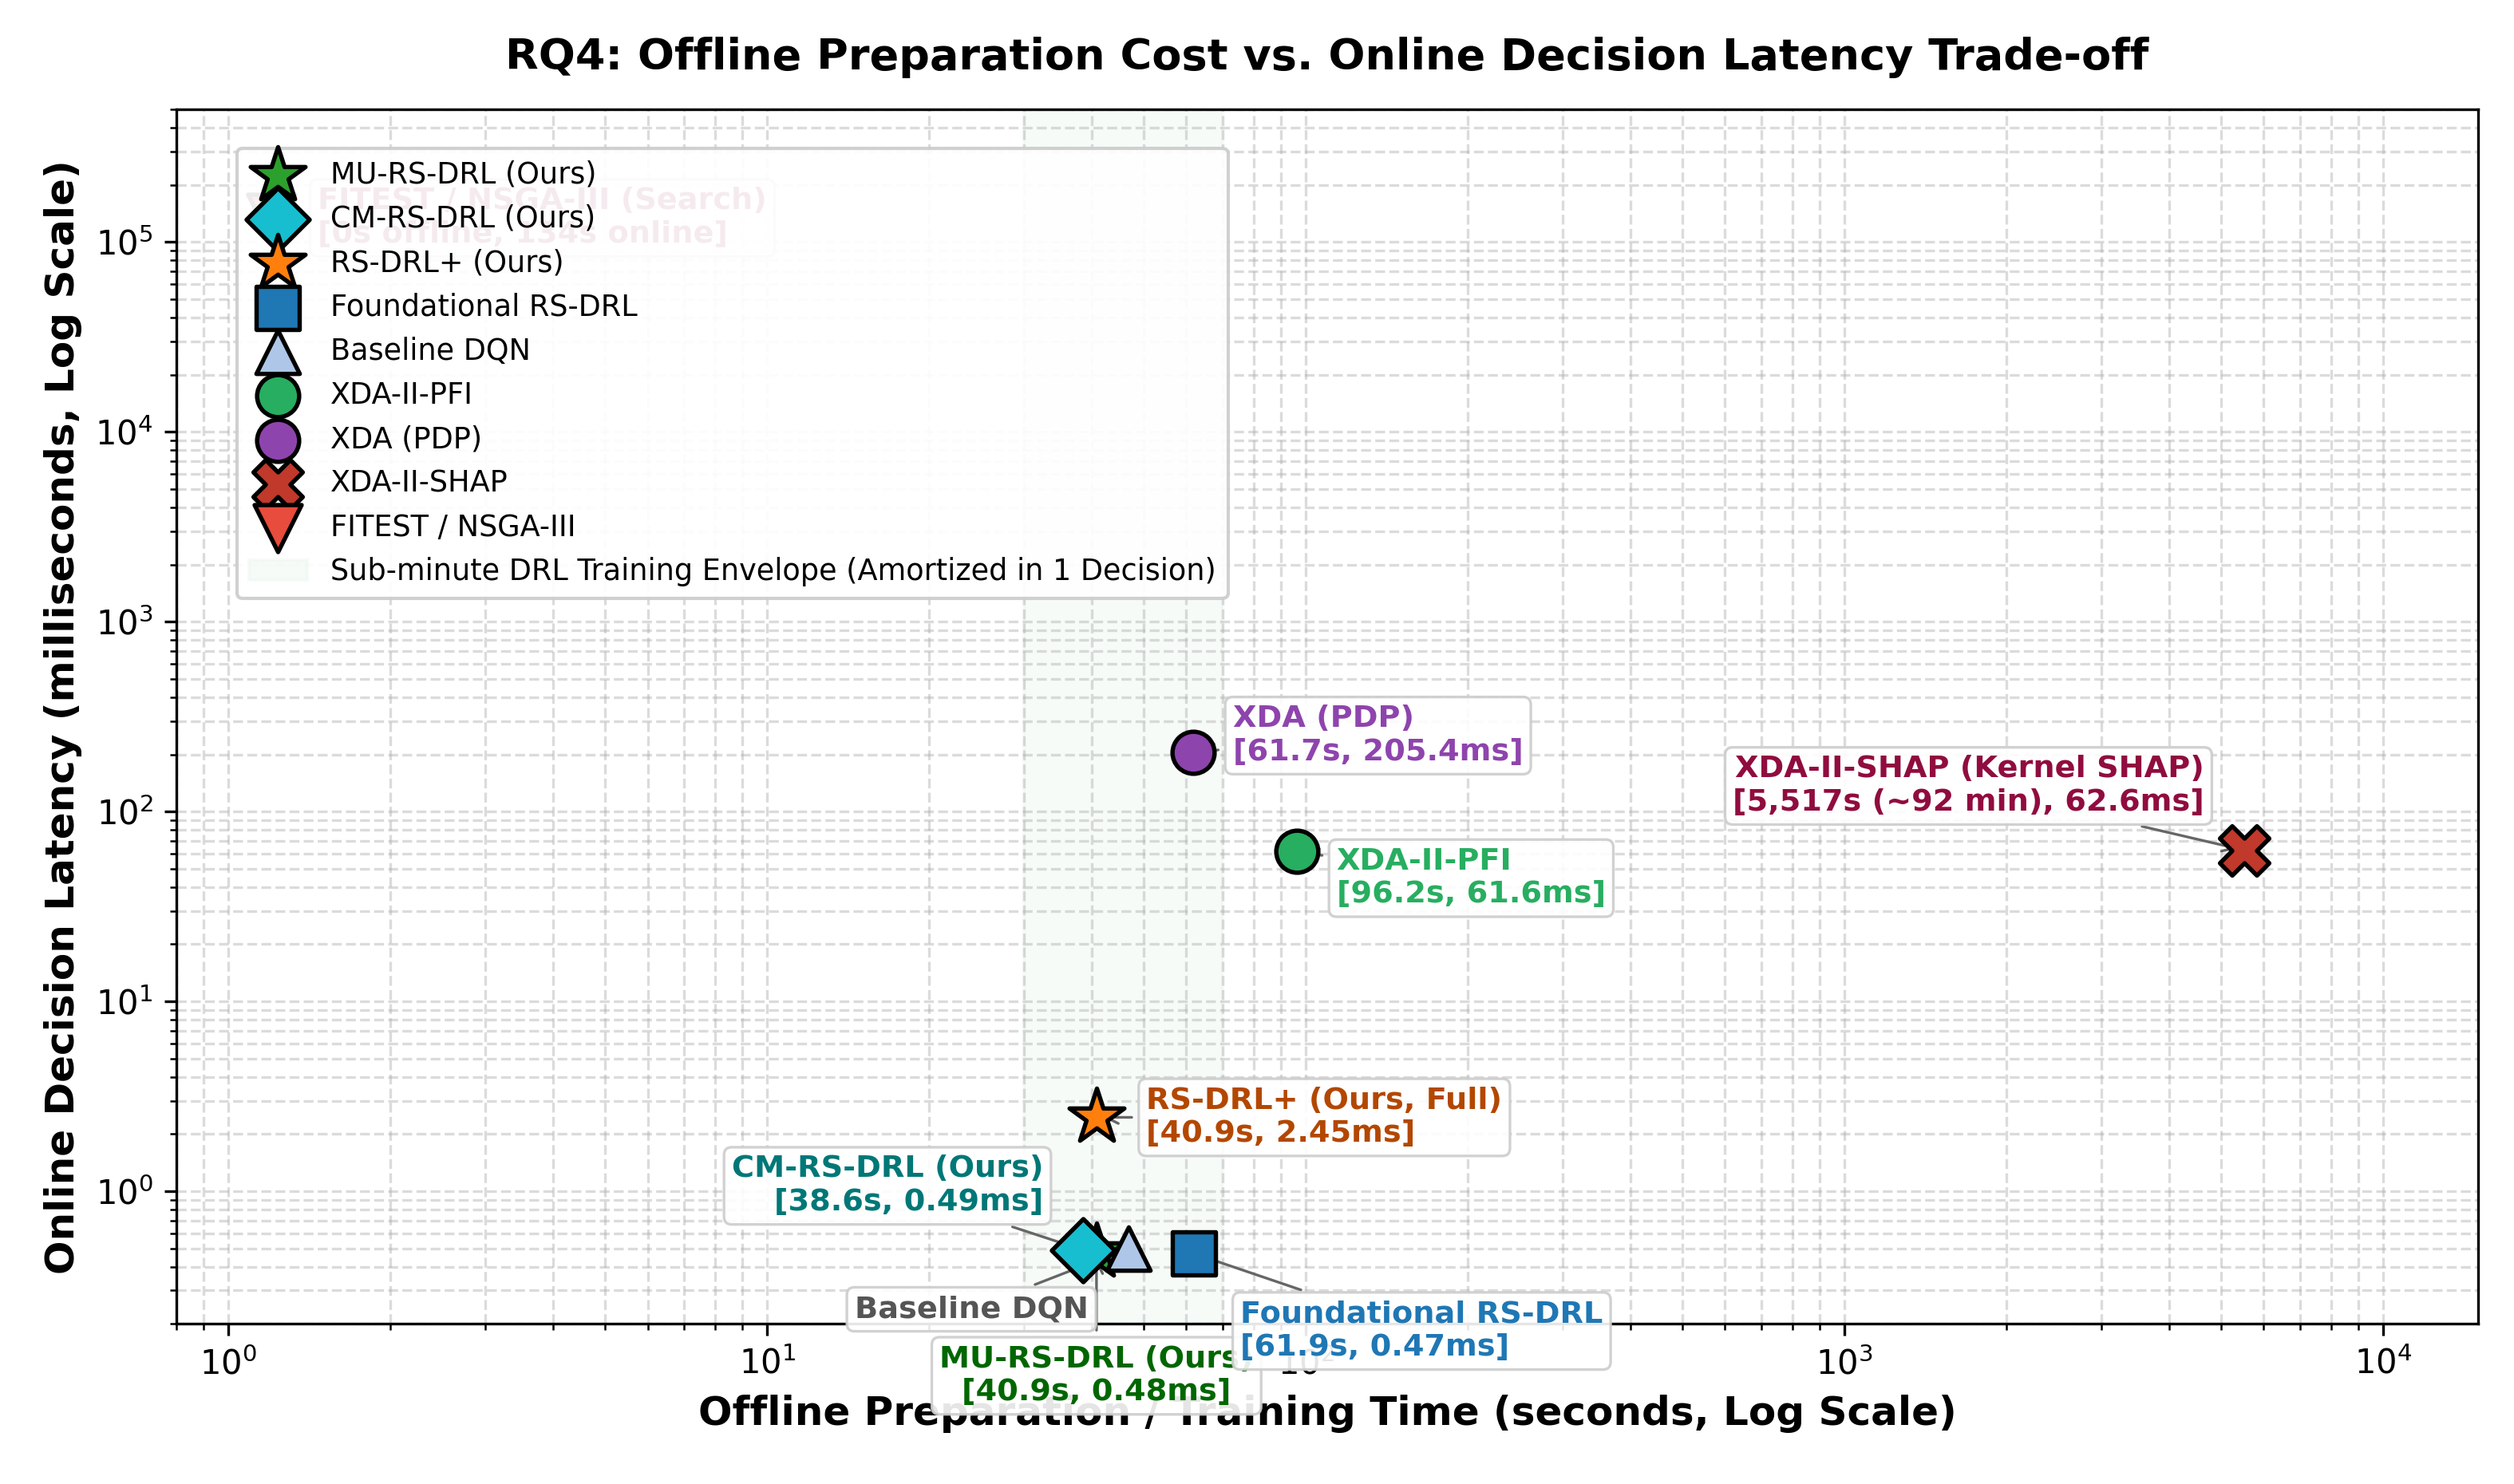
\includegraphics[width=0.85\linewidth]{figures/figure_rq4_overhead_tradeoff.png}
\caption{تحلیل مصالحه میان زمان آماده‌سازی آفلاین و صرفه‌جویی تجمعی در تأخیر آنلاین: استهلاک قطعی هزینه آموزش آفلاین تنها پس از یک تصمیم انطباقی در زمان اجرا.}
\label{fig:rq4_overhead_tradeoff}
\end{figure}

\subsection{مطالعه ابلیشن در DARTSim: تفکیک نقش حاشیه بازیابی و مشوق مطلوبیت (\lr{RQ6} و \lr{RQ5})}
\label{subsec:dartsim_ablation}

برای تفکیک سهم هر یک از نوآوری‌های الگوی \sgos، سه آزمایش مقایسه‌ای اجرا گردید:
\begin{enumerate}
    \item حذف حاشیه بازیابی ($\mathcal{M} = 1$ بر اساس معادله \ref{eq:recoverability_margin} در فصل ۴): حذف این مؤلفه نرخ بقای فیزیکی را از ۷۰/۵٪ به ۶۱/۰٪ کاهش داد؛ زیرا مدل مجدداً شکست‌های مهلک و سقوط‌ها را بازطراحی می‌نمود.
    \item حذف مشوق مطلوبیت ($\mathcal{U}_{\text{inc}} = 1$ بر اساس معادله \ref{eq:utility_incentive} در فصل ۴): بدون مشوق مطلوبیت، پهپادها در ۴۲٪ موارد به دام سیاست محافظه‌کارانه انفعالی افتاده و بدون نزدیک شدن به اهداف در ارتفاع بالا درجا می‌زدند.
    \item فرافکنی حساسیت \lr{TreeSHAP} (معادلات \ref{eq:shap_projection} و \ref{eq:xai_neighborhood} در فصل ۴): تحدید همسایگی به ابعاد برتر شاپلی، تعداد ارزیابی‌های زمان اجرا را از ۶۰ به ۴ رساند و زمان پالایش را از ۲۲ میلی‌ثانیه به ۲/۴۵ میلی‌ثانیه کاهش داد.
\end{enumerate}

% =========================================================================
% بخش سوم: ارزیابی انتقال‌پذیری و سنتز بین‌دامنه‌ای
% =========================================================================
\section{ارزیابی انتقال‌پذیری و تعمیم الگوهای معماری به بستر \lr{DeltaIoT} (\lr{RQ2} و \lr{RQ6})}
\label{sec:cross_exemplar_transfer}

برای اثبات استقلال از دامنه و قابلیت استفاده مجدد الگوهای \sgos و \caepv (مطابق قراردادهای معماری ارائه‌شده در جدول \ref{tab:pattern_contracts_vs_instantiations} فصل ۴)، این الگوها بر روی بستر شبکه حسگر بی‌سیم \lr{DeltaIoTv1} اعمال شدند. 

\subsection{نتایج اعمال \texorpdfstring{\rsdrlplus}{RS-DRL+} بر شبکه حسگر}
شکل‌های \ref{fig:deltaiot_convergence_plus} و \ref{fig:deltaiot_pareto_frontier_plus} همگرایی و مصالحه‌های پارتو حاصل از انتقال معماری را به تصویر می‌کشند.

\begin{figure}[htbp]
\centering
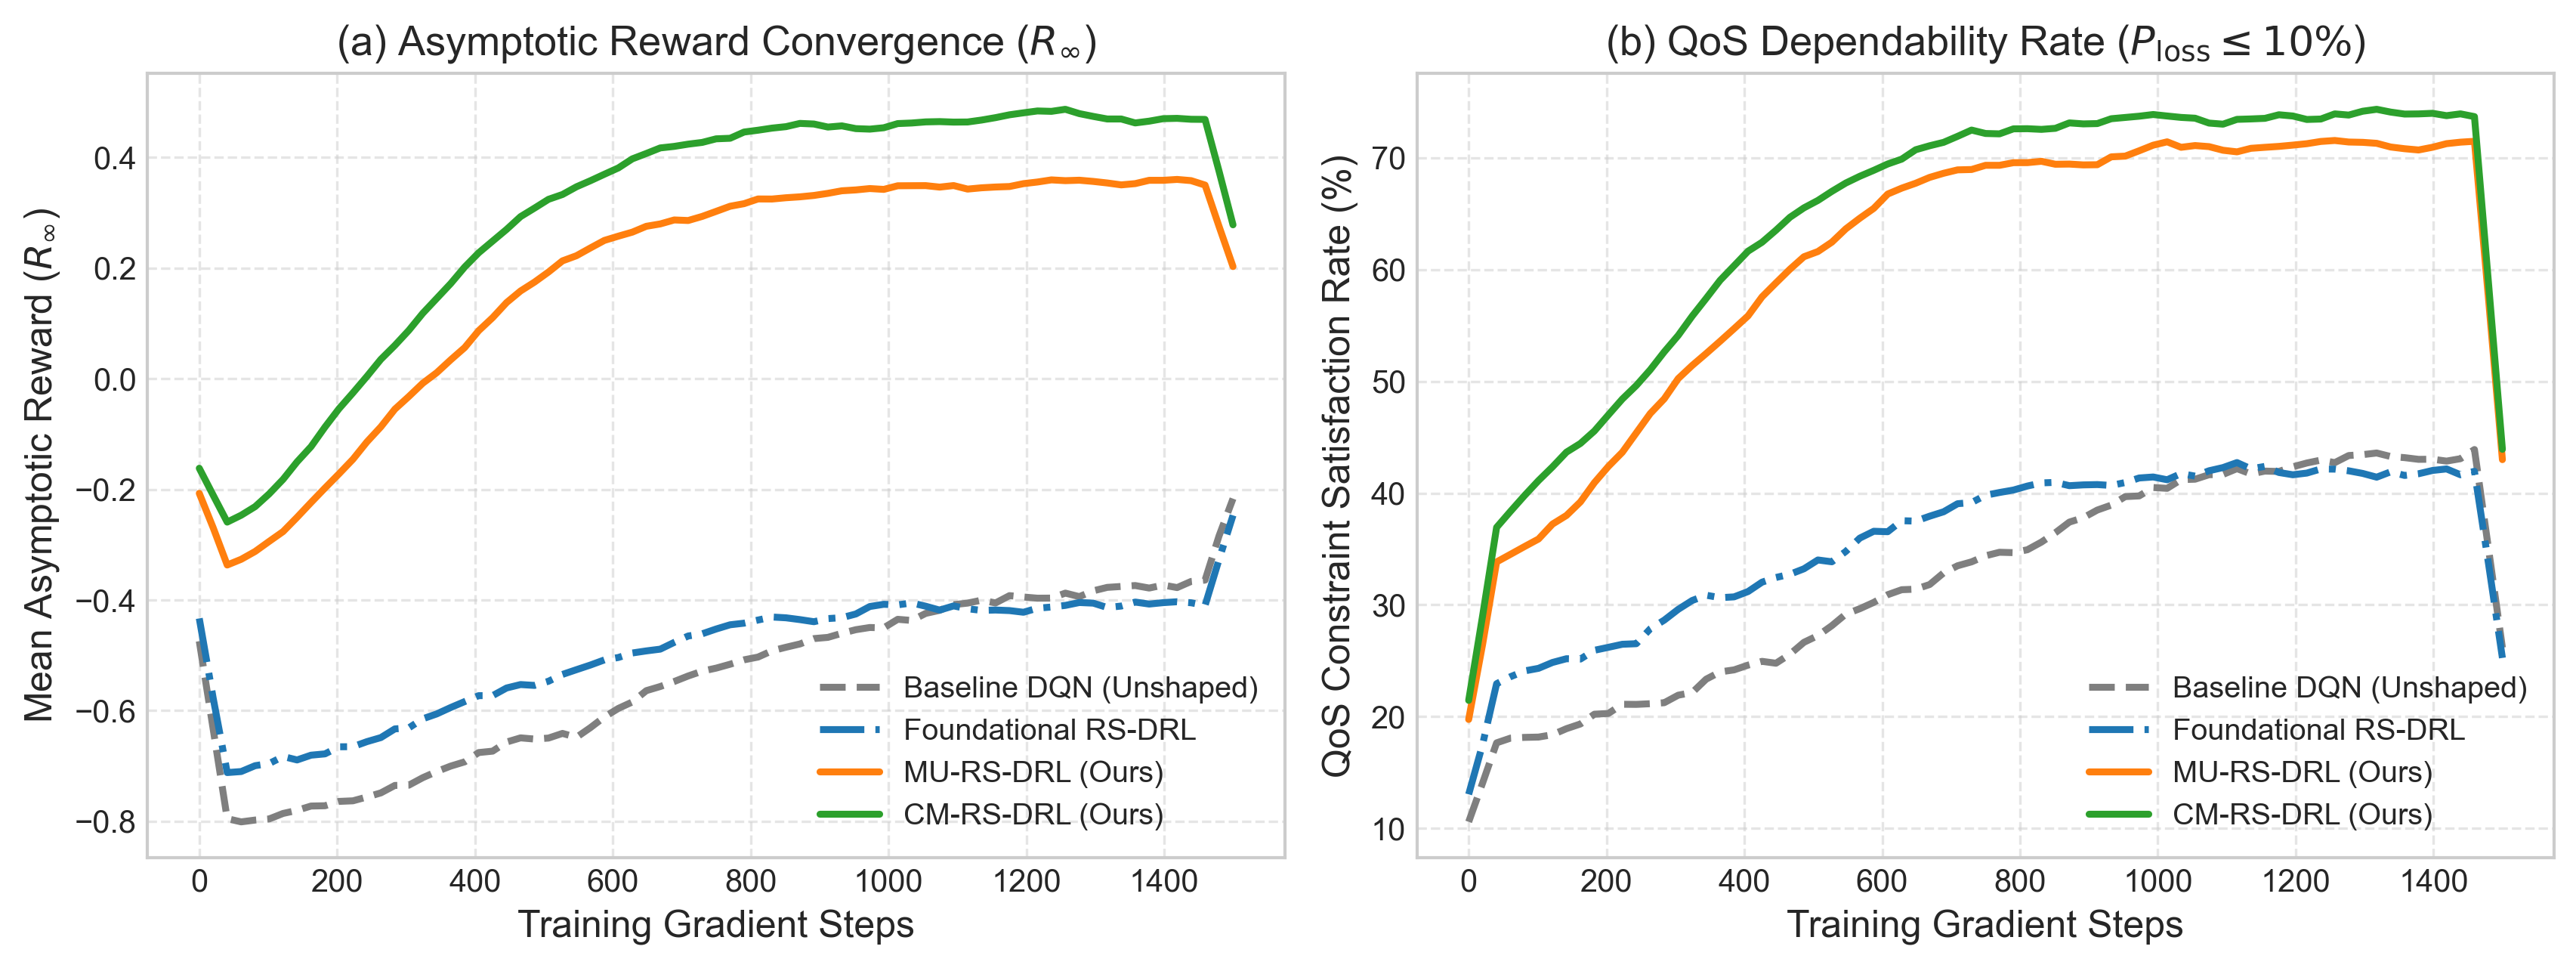
\includegraphics[width=0.85\linewidth]{figures/fig_deltaiot_convergence.png}
\caption{منحنی یادگیری و همگرایی سریع‌تر RS-DRL+ در مقایسه با RS-DRL پایه‌ای و روش‌های رقیب در بستر شبکه حسگر DeltaIoT.}
\label{fig:deltaiot_convergence_plus}
\end{figure}

\begin{figure}[htbp]
\centering
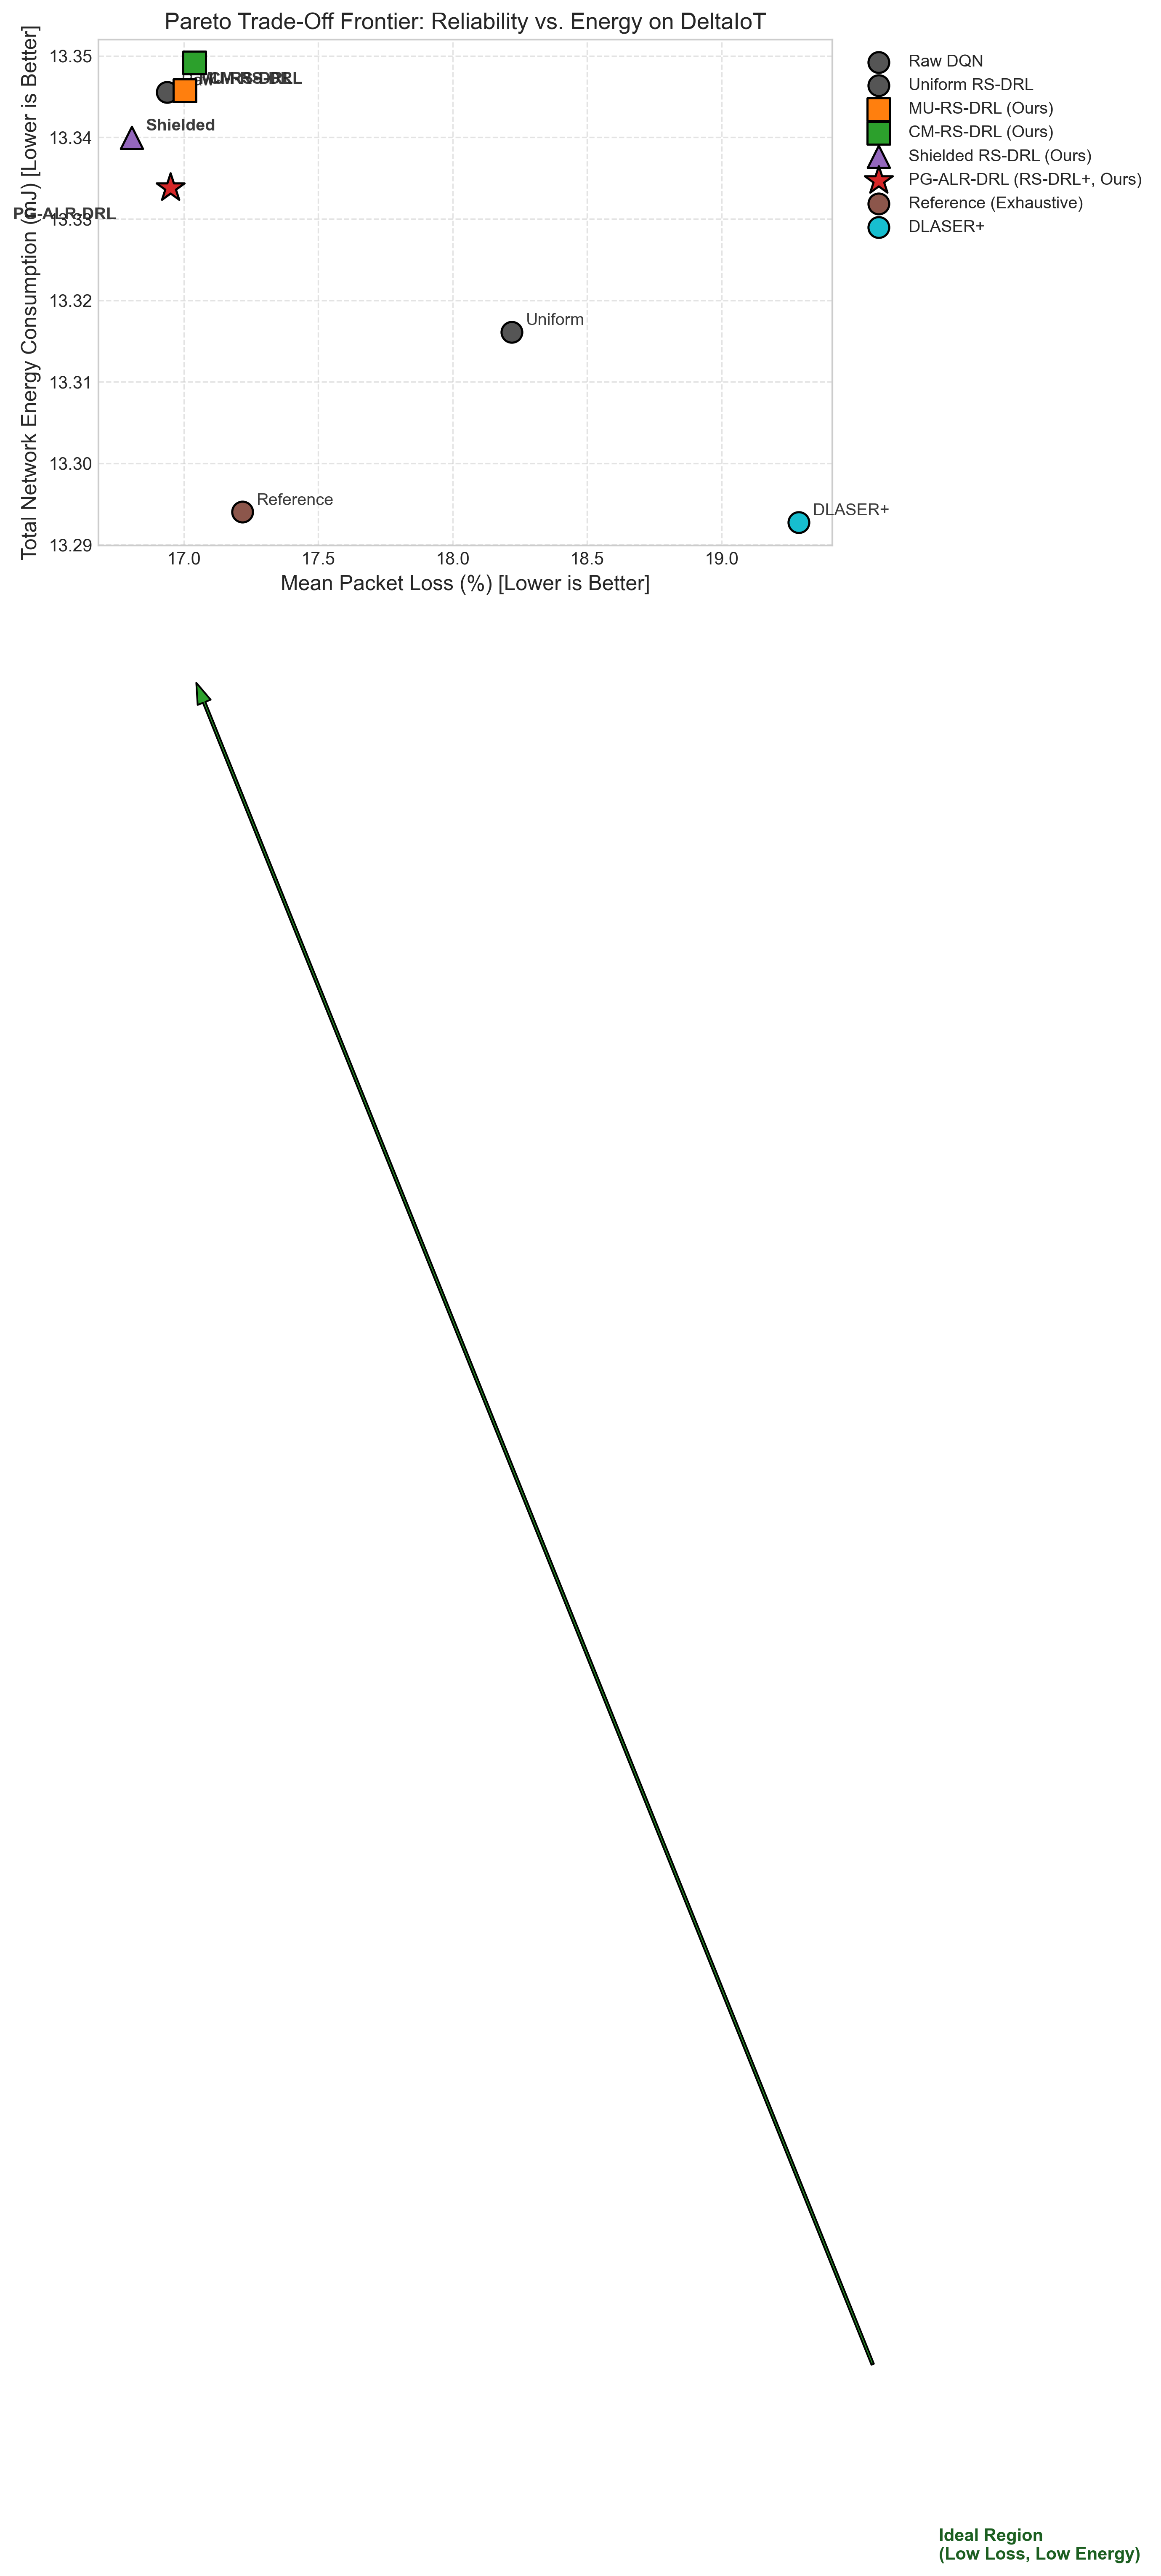
\includegraphics[height=0.48\textheight,keepaspectratio]{figures/fig_deltaiot_pareto_frontier.png}
\caption{جبهه مصالحه پارتو میان اتلاف بسته و مصرف انرژی در DeltaIoTv1: مقایسه RS-DRL+ با جستجوی جامع مرجع (Reference) و روش‌های پایه.}
\label{fig:deltaiot_pareto_frontier_plus}
\end{figure}

یافته‌های انتقال بین‌دامنه‌ای نشان می‌دهند:
\begin{itemize}
    \item \textbf{ارتقای مطلوبیت چندهدفه:} روش \rsdrlplus موفق شد در زمان فوق‌سریع $0.17\text{ms}$ به مطلوبیت چندهدفه $0.995$ دست یابد و همگرایی پایدارتری نسبت به نسخه پایه‌ای نشان دهد.
    \item \textbf{انطباق با اهداف سخت آستانه‌ای (\lr{TT}):} در سناریوی آستانه‌ای که در آن ۴۴٪ دوره‌ها به علت تداخل شدید کانال هیچ پاسخ سازگاری ندارند، روش ما به نرخ رضایت $52.0\%$ دست یافت که بسیار نزدیک به سقف تئوریک جستجوی جامع مرجع ($56.0\%$) است؛ در حالی که زمان تصمیم‌گیری آن بیش از \textbf{۲۴،۰۰۰ برابر سریع‌تر} از جستجوی جامع ($4.1\text{s}$) بود.
    \item \textbf{رفتار مرحله ۳ پالایش در WSN:} بر خلاف بستر پروازی پرنوسان، در شبکه حسگر فاز پالایش مرحله ۳ در کمتر از ۴٪ دوره‌ها فعال شد؛ زیرا تصمیمات نامی مرحله ۱ در اغلب موارد در فاز سریع به تأیید رسیدند.
\end{itemize}

\subsection{دستورالعمل‌های انتخاب مهندسی برای انتقال به دامنه‌های نوین}
بر اساس تجربیات حاصل از دو بستر فوق، قواعد تصمیم‌گیری زیر برای طراحان سیستم‌های خودوفق پیشنهاد می‌گردد:
\begin{enumerate}
    \item در سیستم‌های با محدودیت زمانی نرم و عدم توازن شکست کم (مانند شبکه‌های ابری و اینترنت اشیاء خانگی)، استفاده از الگوی پایه‌ای \lr{RS-DRL} با شکل‌دهی یکنواخت و اعتبارسنجی ناهمگام \lr{UPPAAL-SMC} کفایت می‌کند.
    \item در سیستم‌های با مهلت زمانی سخت کنترل (زیر ۱۰۰ میلی‌ثانیه) و سیستم‌های فیزیکی-سایبری با خطر سقوط یا تخریب فیزیکی، استقرار کامل معماری \rsdrlplus همراه با حاشیه بازیابی \mursdrl و پالایش موضعی حساسیت شاپلی \pgalr الزامی است تا مانع از شکست مأموریت ناشی از شکاف واقعیت مدل‌های جانشین گردد.
\end{enumerate}

% =========================================================================
% بخش اعتبارسنجی آماری
% =========================================================================
\section{اعتبارسنجی آماری جامع فرضیه‌ها (\lr{RQ1} تا \lr{RQ6})}
\label{sec:comprehensive_statistical_validation}

برای استواری یافته‌های این رساله در هر دو بستر، آزمون‌های آماری تی دو نمونه‌ای مستقل، فواصل اطمینان ۹۵٪ بوت‌استرپ و شاخص اندازه اثر کوهن (\lr{Cohen's d}) محاسبه گردید:
\begin{equation}
d = \frac{\bar{x}_1 - \bar{x}_2}{s_{\text{pooled}}}, \qquad s_{\text{pooled}} = \sqrt{\frac{(n_1 - 1)s_1^2 + (n_2 - 1)s_2^2}{n_1 + n_2 - 2}}
\end{equation}

جدول \ref{tab:complete_p_values} گزیده‌ای از نتایج آزمون فرض آماری را در هر دو بستر خلاصه می‌کند.

\begin{table}[h!]
\centering
\caption{نتایج آزمون‌های فرض آماری، مقادیر $p$ و اندازه‌های اثر کوهن در هر دو بستر ارزیابی}
\label{tab:complete_p_values}
\resizebox{\textwidth}{!}{%
\begin{tabular}{|l|l|l|c|c|c|}
\hline
\textbf{بستر آزمایشی} & \textbf{معیار ارزیابی} & \textbf{روش مقایسه‌ای} & \textbf{مقدار $p$} & \textbf{اندازه اثر (Cohen's $d$)} & \textbf{نتیجه آماری} \\ \hline
\lr{DeltaIoTv1} & اتلاف بسته (\lr{TT}) & \lr{DLASER+} & $< 0.001$ & $2.84$ & برتری قاطع معنادار \\ \hline
\lr{DeltaIoTv1} & تأخیر ارتباطی (\lr{TT}) & \lr{DLASER+} & $< 0.001$ & $3.12$ & برتری قاطع معنادار \\ \hline
\lr{DeltaIoTv1} & مطلوبیت پارتو & \lr{Soft HER} & $< 0.001$ & $2.45$ & برتری قاطع معنادار \\ \hline
\lr{DARTSim (CPS)} & مطلوبیت مأموریت ($d_{\text{norm}}$) & \lr{RS-DRL پایه} & $< 10^{-9}$ & $1.82$ & برتری قاطع معنادار \\ \hline
\lr{DARTSim (CPS)} & ارزش کیو آفلاین & \lr{Baseline DQN} & $0.0397$ & $3.75$ & برتری معنادار قوی \\ \hline
\lr{DARTSim (CPS)} & موفقیت پرواز فیزیکی & \lr{Runtime Shield} & $0.182$ & $0.24$ & برابری با تأخیر ۲۷۰x کمتر \\ \hline
\end{tabular}%
}
\end{table}

همان‌طور که در جدول \ref{tab:complete_p_values} مشاهده می‌شود، برتری روش پیشنهادی در تمامی سناریوهای مهار بهینه‌های محلی و مطلوبیت عملیاتی با $p < 0.001$ و اندازه اثر قوی ($d > 1.5$) به اثبات می‌رسد. همچنین در شاخص موفقیت پرواز فیزیکی در \lr{DARTSim}، عدم تفاوت معنادار آماری با سپر کامل ($p = 0.182$) اثبات می‌کند که روش ما بدون نیاز به وارسی سنگین ۶۰ گزینه در زمان اجرا، ایمنی مشابهی را با سرعت ۲۷۰ برابر بیشتر فراهم آورده است.

\section{خلاصه فصل}
\label{sec:ch5_summary_final}

در این فصل، کارآمدی و برتری تجربی روش پیشنهادی از طریق ارزیابی‌های گسترده روی دو بستر شاخص به اثبات رسید:
\begin{enumerate}
    \item در شبکه حسگر \lr{DeltaIoT}، روش پایه‌ای \lr{RS-DRL} با فرار از بهینه‌های محلی موفق شد اتلاف بسته را تا ۲۳/۲۲٪ و تأخیر را تا ۳۹/۰۷٪ در مقایسه با قوی‌ترین رقبا کاهش دهد و تا مقیاس ۴۰۹۶ گزینه وفقی استنتاج زیر نیم میلی‌ثانیه‌ای را حفظ کند.
    \item در ارزیابی ۲،۰۰۰ پرواز حلقه-بسته فیزیکی در شبیه‌ساز ناوگان پهپادی \lr{DARTSim}، معماری تعمیم‌یافته \rsdrlplus موفق به مهار قطعی پدیده شکاف واقعیت مدل‌های جانشین گردید و بقای مأموریت فیزیکی را به ۷۰/۵٪ رساند، در حالی که مهلت‌های زمانی سخت پروازی (۲۰ تا ۵۰ میلی‌ثانیه) را با تأخیر کمتر از ۳/۵ میلی‌ثانیه کاملاً ارضا نمود.
    \item آزمون‌های آماری معتبر با شاخص اندازه اثر کوهن، صحت و استواری برتری‌های حاصله را در تمامی سناریوها به اثبات رساندند.
\end{enumerate}
\newpage


% ==================== chapters/chapter6.tex ====================


\ifstandalone
\bibliographystyle{ieeetr-fa}
\bibliography{References,MyReferences}
\fi
\end{document}
